% Copyright 2008 by Christian Feuersaenger
%
% This file may be distributed and/or modified
%
% 1. under the LaTeX Project Public License and/or
% 2. under the GNU Free Documentation License.
%
% See the file doc/generic/pgf/licenses/LICENSE for more details.
\section{Externalization Library}
{
\pgfkeys{
	/pdflinks/search key prefixes in/.add={/tikz/external/,}{}
}
\label{section-libs-external}
{\noindent {\emph{by Christian Feuers\"anger}}}

\begin{tikzlibrary}{external}
	This library provides a high-level automatic or semi--automatic export feature for \tikzname\ pictures.
	Its purpose is to convert each picture to a separate \pdf\ without changing the document as such.

	It also externalizes |\label|  information (and other aux file related stuff) using auxiliary files.
\end{tikzlibrary}

\subsection{Overview}

There are several reasons why external images for at least some pictures are of interest:
\begin{enumerate}
	\item Larger picture require a considerable amount of time, which is necessary for every compilation. However, only few images will change from run to run. It can simply save time to export finished images and include them as final graphics.
	\item It may be desirable to have final images for some graphics, for example to include them in third--party programs or to communicate them electronically.
	\item It may be necessary to typeset a file in environments where \pgfname\ and \tikzname\ are not available. In this case, external images are the only way to ensure compatibility.
\end{enumerate}
The purpose of this library is to provide a way to export any \tikzname-picture to separate \pdf\ (or \eps) images without changing the main document. It is actually a simple user interface to the |\beginpgfgraphicnamed| $\dotsc$ |\endpgfgraphicnamed| framework of \pgfname\ which is discussed in section~\ref{section-external}.

\subsection{Requirements}
For most users, the library does not need special attention since requirements are met anyway. It collects all tokens between |\begin{tikzpicture}| and the next following |\end{tikzpicture}| and replaces them by the appropriate graphics or it takes steps to generate such an image.% For Con\TeX t and plain \TeX\ users, the appropriate begin and end picture statements apply.

It can't expand macros during this step, so the only requirement is that every picture's end is directly reachable from its beginning, without further macro expansion. Furthermore, the library assumes that all \LaTeX\ pictures are ended with |\end{tikzpicture}|.% In Con\TeX t, the end command is assumed to be |\stoptikzpicture| and for plain \TeX\ it is |\endtikzpicture|.

The library always searches for the \emph{next} picture's end, |\end{tikzpicture}|. As a consequence, you can't use nested pictures directly. You \emph{can} nest pictures, but you have to avoid that the nested picture's |\end| command is found before the outer |\end| command (for example using bracing constructs or by writing the nested picture into a separate macro call).

Consider using the |\tikzexternaldisable| method in case you'd like to skip selected pictures which do not meet the requirements.

\subsection{A Word About Con\TeX t And Plain \TeX}
Currently, the basic layer backend |\beginpgfgraphicnamed| $\dotsc$ |\endpgfgraphicnamed| relies on \LaTeX\ only, so externalization is currently only supported for \LaTeX.
%The library comes in three different versions, one for \LaTeX, one for Con\TeX t and one for plain \TeX. For reasons of simplicity, examples in this manual only refer to \LaTeX\ (especially |pdflatex|).

\subsection{Externalizing Graphics}
After loading the library, a call to |\tikzexternalize| is necessary to activate the externalization.
\begin{codeexample}[code only]
\documentclass{article}
% main document, called main.tex
\usepackage{tikz}

\usetikzlibrary{external}
\tikzexternalize % activate!

\begin{document}
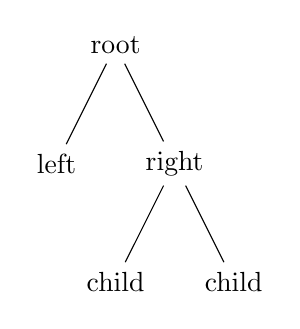
\begin{tikzpicture}
  \node {root}
    child {node {left}}
    child {node {right}
      child {node {child}}
      child {node {child}}
    };
\end{tikzpicture}

A simple image is \tikz \fill (0,0) circle(5pt);.
\end{document}
\end{codeexample}

The method works as follows: if the document is typeset normally, the library searches for replacement images for every picture. Filenames are generated automatically in the default configuration. In our case, the two file names will be |main-figure0| and |main-figure1|. If they exist, those images are simply included and the pictures as such are not processed. If graphics files do not exist, steps are taken to generate the missing ones. Since (currently) only one output file can be set, each missing image needs to be generated by a separate run of \LaTeX\ in which the |\jobname| is set to the desired image file name.
In the default configuration |mode=convert with system call|, these commands are issued automatically by using the |\write18| method to call system commands. It is also possible to output every required file name or to generate a |makefile|; users will need to issue the required commands manually (or with |make|). The probably most comfortable way is to use the default configuration with
\begin{codeexample}[code only, tikz syntax=false]
pdflatex -shell-escape main
\end{codeexample}
\noindent which authorizes |pdflatex| to call itself recursively to generate the images. When it finishes, all images are generated and the document already includes them.


From this point on, successive runs of \LaTeX\ will use the final graphics files, the pictures won't be used anymore. Section~\ref{section-libs-external-nopgf} contains details about how to submit such a file to environments where \pgfname\ is not available.

\begin{command}{\tikzexternalize\oarg{optional arguments}}
	This command activates the externalization. It installs commands to replace every \tikzname-picture. It needs to be called before |\begin{document}| because it may need to install its separate shipout routine.


	The \meta{optional arguments} can be any of the keys described below.

	Note that the generation/modification of auxiliary files like |.aux|, |.toc| etc.\ is usually suppressed while a single image is externalized (details for |\label| support follow).

	It is also possible to write |\tikzexternalize|\marg{main job name} if the argument is delimited by curly braces. This case is mainly for backwards compatibility and is no longer necessary. Since it might be useful in rare circumstances, it is documented in section~\ref{sec:external:detail}.

	A detailed description about the process of externalization is provided in section~\ref{sec:external:detail}.

	\begin{command}{\tikzexternalrealjob}%
		After the library is loaded, this macro will \emph{always} contain the correct main job's name (in the example above, it is |main|). It is to be used instead of |\jobname| when the externalization is in effect.
	\end{command}
	\begin{command}{\pgfactualjobname}
		Once |\tikzexternalize| has been called, |\pgfactualjobname| contains the name of the currently generated output file (which may be |main| or |main-figure0| or |main-figure1| in our example above).
	\end{command}
	\begin{command}{\jobname}
		The value of |\jobname| is one of |\tikzexternalrealjob| or |\pgfactualjobname|, depending on the configuration. In short: if auxiliary file support (|\label| and |\ref|) is activated, |\jobname=\tikzexternalrealjob| (since that's the base file name of auxiliary files).
	\end{command}
\end{command}

\begin{key}{/tikz/external/system call=\marg{template}}
\label{extlib:systemcall:option}
	A template string used to generate system calls. Inside of \marg{template}, the macro |\image| can be used as placeholder for the image which is about to be generated while |\texsource| contains the main file name (in truth, it contains |\input|\marg{main file name}, but that doesn't matter).

	The default is
\begin{codeexample}[code only]
\tikzset{external/system call={pdflatex \tikzexternalcheckshellescape -halt-on-error
    -interaction=batchmode -jobname "\image" "\texsource"}
\end{codeexample}
	\noindent where \declareandlabel{\tikzexternalcheckshellescape} inserts the value of the configuration key |shell escape|
	if and only if the current document has been typeset with |-shell-escape|\footnote{Note that this is always true for the default configuration. This security consideration applies mainly for \texttt{mode=list and make} which will also work \emph{without} shell escapes.}.

	For |eps| output, you can (and need to) use
\begin{codeexample}[code only, tikz syntax=false]
\tikzset{external/system call={latex \tikzexternalcheckshellescape -halt-on-error
    -interaction=batchmode -jobname "\image" "\texsource";
    dvips -o "\image".ps "\image".dvi}}
\end{codeexample}
	
	The argument \marg{template} will be expanded using |\edef|, so any control sequences will be expanded. During this evaluation, `|\\|' will result in a normal backslash, `|\|'. Furthermore, double quotes `|"|', single quotes `|'|', semicolons and dashes `|-|' will be made to normal characters if any package uses them as macros. This ensures compatibility with the |german| package, for example.
\end{key}

\begin{key}{/tikz/external/shell escape=\marg{command-line arg} (initially -shell-escape)}
	Contains the command line option for |latex| which enables the |\write18| feature. For \TeX-Live, this is |-shell-escape|. For Mik\TeX, you should use |\tikzexternalize[shell escape=-enable-write18]|.
\end{key}

\subsubsection{Support for Labels and References In External Files}
The |external| library comes with extra support for |\label| and |\ref| (and other commands which usually store information in the |.aux| file) inside an external files.

There are, however, some points which need your attention when you try to use
\begin{enumerate}
	\item[a)] |\ref| to something in the main document inside an externalized graphics or
	\item[b)] |\label| in the externalized graphics which is referenced in the main document.
\end{enumerate}

For point a), a |\ref| inside of an externalized graphics works \emph{only} if you issue the required system call \emph{manually} or by |make|. The initial configuration |mode=convert with system call| does \emph{not} support |\ref|. But you can copy--paste the system call generated by |mode=convert with system call| and issue it manually. The reason is that |\ref| information is stored in the main |.aux| file -- but this auxiliary file is not completely written when |mode=convert with system call| is invoked (there is a race condition). Note that |\pageref| is not supported (sorry). Thus: if you have |\ref| inside of external graphics, consider using |mode=list and make| or copy--paste the system call for the image(s) and issue it manually.

Point b) is realized automatically by the external library. In detail, a |\label| inside of an externalized graphics causes the external library to generate separate auxiliary files for every external image. These files are called \meta{imagename}|.dpth|. The extension |.dpth| indicates that the file also contains the image's depth (the |baseline| key of \tikzname). Furthermore, anything which would have been written to an |.aux| file will be redirected to the |.dpth| file -- but only things which occur inside of the externalized |tikzpicture| environment. When the main document loads the image, it will copy the |.dpth| file into the main |.aux| file. Then, successive compilations of the main document contain the external |\label| information. In other words, a |\label| in an external graphics needs the following work flow:
\begin{enumerate}
	\item The external graphics needs to be generated together with its |.dpth| (usually automatically by \tikzname).
	\item The main document includes the external graphics and copies the |.dpth| content into its main |.aux| file.
	\item The main document needs to be translated once again to re-read its |.aux| file\footnote{Note that it is not possible to activate the content of an auxiliary file after \texttt{\textbackslash begin\{document\}} in \LaTeX.}.
\end{enumerate}
There is just one special case: if a |\label|/|\ref| combination is realized itsself by a |tikzpicture| which should be externalized, you need to proceed as for case a) since |mode=convert with system call| can't handle that stuff on its own. Thus, |\label| works automatically, just translate the main document often enough.
\begin{key}{/tikz/external/aux in dpth=\marg{boolean} (initially true)}
	Allows to disable the feature. Disabling it will safe one |\newwrite| command, i.e.\ a write register.

	Also see the |disable dependency files| feature.
\end{key}



\subsubsection{Customizing the Generated File Names}
The default filename for externalized graphics is `\meta{real file name}|-figure_|\meta{number}' where \meta{number} ranges from $0$ to whatever is required. However, there are a couple of ways to change the generated filenames:
\begin{itemize}
	\item Changing the overall file name using a |prefix|,
	\item Changing the file name for a single figure using |\tikzsetnextfilename|,
	\item Changing the file name for a restricted set of figures using |figure name|.
\end{itemize}

\begin{key}{/tikz/external/prefix=\marg{file name prefix} (initially empty)}
	A shortcut for |\tikzsetexternalprefix|\marg{file name prefix}, see below.
\end{key}

\begin{command}{\tikzsetexternalprefix\marg{file name prefix}}
	Assigns a common prefix used by all file names. For example,
\begin{codeexample}[code only]
\tikzsetexternalprefix{figures/}
\end{codeexample}
	will prepend |figures/| to every external graphics file name.

	Please note that |\tikzsetexternalprefix| is the \emph{only} way to assign a prefix in case you want to prepare your document for environments where \pgfname\ is not installed (see section~\ref{section-libs-external-nopgf}).
\end{command}

\begin{command}{\tikzsetnextfilename\marg{file name}}
	Sets the file name for the \emph{next} \tikzname\ picture or |\tikz| short command. It will \emph{only} be used for the next picture.

	Pictures for which no explicit file name has been set (or the next file name is empty) will get automatically generated file names.

	Please note that |prefix| will still be prepended to \marg{file name}.
\begin{codeexample}[code only]
\documentclass{article}
% main document, called main.tex
\usepackage{tikz}

\usetikzlibrary{external}
\tikzexternalize[prefix=figures/] % activate

\begin{document}

\tikzsetnextfilename{trees}
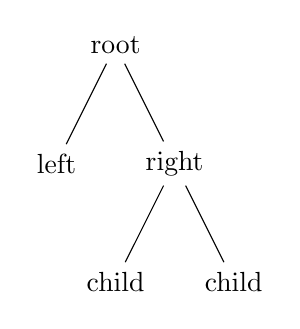
\begin{tikzpicture} % will be written to 'figures/trees.pdf'
  \node {root}
    child {node {left}}
    child {node {right}
      child {node {child}}
      child {node {child}}
    };
\end{tikzpicture}

\tikzsetnextfilename{simple}
A simple image is \tikz \fill (0,0) circle(5pt);. % will be written to 'figures/simple.pdf'


\begin{tikzpicture} % will be written to 'figures/main-figure0.pdf'
   \draw[help lines] (0,0) grid (5,5);
\end{tikzpicture}
\end{document}
\end{codeexample}
\begin{codeexample}[code only, tikz syntax=false]
pdflatex -shell-escape main
\end{codeexample}
\end{command}

\begin{key}{/tikz/external/figure name=\marg{name}}
	Same as |\tikzsetfigurename|\marg{name}.
\end{key}
\begin{command}{\tikzsetfigurename\marg{name}}
	Changes the names of \emph{all} following figures. It is possible to change |figure name| during the document either using |\tikzset{external/figure name|=\marg{name}|}| or with this command. A unique counter will be used for each different \marg{name}, and each counter will start at $0$.

	The value of |prefix| will be applied after |figure name| has been evaluated.
\begin{codeexample}[code only]
\documentclass{article}
% main document, called main.tex
\usepackage{tikz}

\usetikzlibrary{external}
\tikzexternalize % activate

\begin{document}

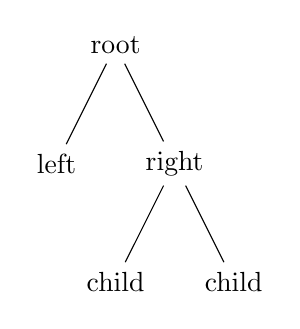
\begin{tikzpicture} % will be written to 'main-figure0.pdf'
  \node {root}
    child {node {left}}
    child {node {right}
      child {node {child}}
      child {node {child}}
    };
\end{tikzpicture}

{
  \tikzsetfigurename{subset_}
  A simple image is \tikz \fill (0,0) circle(5pt);. % will be written to 'subset_0.pdf'

  
\begin{tikzpicture} % will be written to 'subset_1.pdf'
     \draw[help lines] (0,0) grid (5,5);
  \end{tikzpicture}
}% here, the old file name will be restored:

\begin{tikzpicture} % will be written to 'main-figure1.pdf'
   \draw (0,0) -- (5,5);
\end{tikzpicture}
\end{document}
\end{codeexample}
	The scope of |figure name| ends with the next closing brace.

	Remark: Use |\tikzset{external/figure name/.add={prefix_}{_suffix_}}| to add a |prefix_| and a |_suffix_| to the actual value of |figure name|.
\end{command}

\begin{command}{\tikzappendtofigurename\marg{suffix}}
	Appends \meta{suffix} to the actual value of |figure name|.

	It is a shortcut for |\tikzset{external/figure name/.add={}|\marg{suffix}|}| (a shortcut which is also supported if \tikzname\ is not installed, see below).
\end{command}


\subsubsection{Remaking Figures or Skipping Figures}
\begin{command}{\tikzpicturedependsonfile\marg{file name}}
	Adds a dependency for the \emph{next} picture which is about to be externalized. If the command is invoked within a picture environment, it adds a dependency for the surrounding picture. Dependencies are written into \meta{target file}|.dep| in the format
	
	\meta{target file}|.\tikzexternalimgextension: |\meta{file name}.

	The effect is that if \meta{file name} changes, the external graphics associated with the picture shall be remade.

	This command uses the contents of \declareandlabel{\tikzexternalimgextension} to check for graphics. If you encounter difficulties with image extensions, consider redefining this macro (after |\tikzexternalize|).

	\paragraph{Limitations:} this command is currently only supported for |mode=list and make| and the generated |makefile|.
\end{command}
\begin{command}{\tikzexternalfiledependsonfile\marg{external graphics}\marg{file name}}
	A variant of |\tikzpicturedependsonfile| which adds a dependency for an \meta{external graphics}. The argument \meta{external graphics} must be the path as it would have been generated by the external library, i.e.\ without file extension but including any prefixes.
\end{command}
\begin{key}{/tikz/external/disable dependency files}
	Allows to (irreversibly) disable the generation of file dependencies. Disabling it will safe one |\newwrite| command, i.e.\ a write register. Note that the write register is only allocated if the feature has been used at all. This key needs to be provided as argument to |\tikzexternalize| (or it needs to be set before calling |\tikzexternalize|).

	Also see the |aux in dpth| key.
\end{key}

\begin{key}{/tikz/external/force remake=\marg{boolean} (default true)}
	A boolean which is used to customize the up-to-date checks of all following figures. Every up-to-date check will fail, resulting in automatic regeneration of every following figure.

\begin{codeexample}[code only]
\tikzset{external/force remake}

\begin{tikzpicture}
	\draw (0,0) circle(5pt);
\end{tikzpicture}
\end{codeexample}
	You can also use |force remake| inside of a local \TeX\ group to remake only selected pictures. The example
\begin{codeexample}[code only]
\tikz \draw (0,0) -- (1,1);

{
\tikzset{external/force remake}

\begin{tikzpicture}
   \draw (0,0) circle(5pt);
\end{tikzpicture}
}

\tikz \draw (0,0) -- (1,1);
\end{codeexample}
	will only apply |force remake| to the second figure.

	Up-to-date checks are applied for |mode=convert with system call| and the makefile generated by |mode=list and make|.
\end{key}

\begin{key}{/tikz/external/remake next=\marg{boolean} (default true)}
	A variant of |force remake| which applies only to the next image.
\end{key}

\begin{key}{/tikz/external/export next=\marg{boolean} (default true)}
	A boolean which can be used to disable the export mechanism for single pictures.
\end{key}

\begin{key}{/tikz/external/export=\marg{boolean} (initially true)}
	A boolean which can be used to disable the export mechanism for all pictures inside of the current \TeX-scope.

\begin{codeexample}[code only]
\begin{document}
\begin{tikzpicture} % will be exported
	...
\end{tikzpicture}

{
\tikzset{external/export=false}
\begin{tikzpicture} % won't be exported
	...
\end{tikzpicture}
...
}

\begin{tikzpicture} % will be exported
	...
\end{tikzpicture}
\end{document}
\end{codeexample}
	For \LaTeX, the feature lasts until the next |\end|\marg{$\cdot$} (this holds for every call to |\tikzset|).
\end{key}

\begin{key}{/tikz/external/up to date check=\marg{choice} (initially md5)}
	The |external| lib has to decide when some existing figure is up-to-date. In such a case, it can be used without remaking it. Outdated pictures will be remade.

	The key |up to date check| allows to choose among a couple of heuristics which are supposed to catch the most important reasons to remake a figure.

	The |up to date check| can be overrule by any of the |force remake| or |remake next| keys: if one of them is true, the figure is not up-to-date. 

	The choice \declare{simple} is based on the existence of the file: the file is
	up-to-date if and only if it exists.
	
	The choice \declare{md5} generates an MD5 checksum of the picture for which the up-to-date check is running. The MD5 is compared against the MD5 of the previous run, which, in turn, will be written into an extra file with the extension |.md5|. This file will be modified if and only if the MD5 comparison indicates a difference. The MD5 computation is based on the pdf\TeX\ method |\pdfmdfivesum|. If it is unavailable for some reason, the choice |diff| will be used instead.

	The choice \declare{diff} is the same as MD5 -- except that it compares the picture content as-is instead of a hash. The |.md5| file will be used to compare an old version with the current one -- but its content is some ``normalized'' version of the picture for internal use.

	\paragraph{Attention:} the content--based strategies |md5| and |diff| operate on the picture content -- and only on the picture content. Here, ``picture content'' only includes the top--level tokens; no expansion is applied and no included files are part of the strategies. If you change preamble styles, you have to rebuild the figures manually (for example by deleting the generated graphics files). If you have include files, consider using |\tikzpicturedependsonfile| and its variants. Since this key provides heuristics, you should always remake your figures before you finally publish your document.

	The |up to date check| is applied for |mode=convert with system call| and |mode=list and make|.
\end{key}

\begin{command}{\tikzexternaldisable}
	Allows to disable the complete externalization. While |export next| will still collect the contents of picture environments, this command uninstalls the hooks for the external library completely. Thus, nested picture environments or environments where |\end{tikzpicture}| is not directly reachable won't produce compilation failures -- although it is not possible to externalize them automatically.

	The externalization remains disabled until the end of the next \TeX\ group (or environment) or until the next call to |\tikzexternalenable|.
\end{command}

\begin{command}{\tikzexternalenable}
	Re-enables a previously running externalization after |\tikzexternaldisable|.
\end{command}


\subsubsection{Customizing the Externalization}
\begin{key}{/tikz/external/figure list=\marg{boolean} (initially true)}
	A boolean which configures whether a figure list shall be generated. A figure list is an output file named \marg{jobname}|.figlist| which is filled with file names of each figure, one per line.

	This file is not used by \TeX\ anymore, its purpose is to issue the required conversion commands |pdflatex -jobname |\marg{picture file name} \marg{main file} manually (or in a script). See section~\ref{sec:external:detail} for the details about the expected system call (or activate |mode=convert with system call| and inspect your log file).

\begin{codeexample}[code only]
\documentclass{article}
% main document, called main.tex
\usepackage{tikz}

\usetikzlibrary{external}
\tikzexternalize[
   mode=graphics if exists,
   figure list=true,
   prefix=figures/]

\begin{document}

\tikzsetnextfilename{trees}
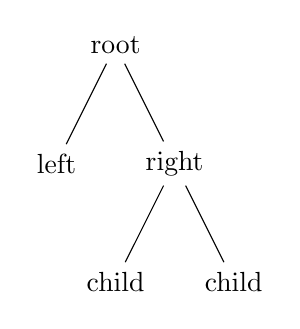
\begin{tikzpicture}
  \node {root}
    child {node {left}}
    child {node {right}
      child {node {child}}
      child {node {child}}
    };
\end{tikzpicture}

\tikzsetnextfilename{simple}
A simple image is \tikz \fill (0,0) circle(5pt);.


\begin{tikzpicture}
   \draw[help lines] (0,0) grid (5,5);
\end{tikzpicture}
\end{document}
\end{codeexample}

\begin{codeexample}[code only, tikz syntax=false]
pdflatex main
\end{codeexample}
generates |main.figlist| containing
\begin{codeexample}[code only, tikz syntax=false]
figures/trees
figures/simple
figures/main-figure0
\end{codeexample}
\end{key}

\begin{key}{/tikz/external/mode=\marg{choice} (initially convert with system call)}
	Configures what to do with \tikzname\ pictures (unless we are currently externalizing one particular image, in that case, these modes are ignored).

	The preconfigured mode |convert with system call| checks whether external graphics files are up-to-date and includes them if that is the case. Any picture which is not up-to-date will be generated automatically using a system call. The system call can be configured using the |system call| template. The up-to-date check is applied according to the |up to date check| key.
As soon as |convert with system call| is set, the |figure list| will be disabled -- such a file is not required. In case you still need or want it, you can enable it after setting |mode|.

	Please note that system calls may be disabled for security reasons. For pdflatex, they can be enabled using
\begin{codeexample}[code only, tikz syntax=false]
pdflatex -shell-escape
\end{codeexample}
	while other \TeX\ variants may need other switches. The feature is sometimes called |\write18|.
	
	The choice |only graphics| always tries to replace pictures with external graphics. It is an error if the graphics file does not exist.

	The choice |no graphics| (or, equivalently, |only pictures|) typesets \tikzname\ pictures without checking for external graphics.

	A mixture is |graphics if exists|, it checks whether a suitable graphics file exists and includes it if that is the case. If it does not exist, the picture is typeset using \TeX.

	Mode |list only| skips every \tikzname\ picture; it only generates the file \marg{main file}|.figlist| containing file names for every picture, the contents of any picture environment is thrown away and a replacement text is shown. This implies |figure list=true|. See also the |list and make| mode which includes available graphics.

	The mode |list and make| is similar to |list only|: it generates the same file \marg{main file}|.figlist|, but any images which exist already are included as graphics instead of ignoring them. Furthermore, this mode generates an additional file: \marg{main file}.makefile. This allows to use a work flow like
\begin{codeexample}[code only, tikz syntax=false]
% step 1: generate main.makefile:
pdflatex main
% step 2: generate ALL graphics on 2 processors:
make -j 2 main.makefile
% step 3: include the graphics:
pdflatex main
\end{codeexample}
	\noindent This last make method is optional: |list and make| just assumes that images are generated somehow (not necessarily with the generated makefile). The generated makefile allows parallel externalization of graphics on multi-core systems and it supports any file dependencies configured with |\tikzpicturedependsonfile|. Furthermore, it respects the |force remake| and |remake next| keys.


\end{key}


\begin{key}{/tikz/external/verbose IO=\marg{boolean} (initially true)}
	A boolean which configures whether I/O operations shall be listed in the logfile.
\end{key}
\begin{key}{/tikz/external/verbose optimize=\marg{boolean} (initially true)}
	A boolean which configures whether optimization operations shall be listed in the logfile.
\end{key}
\begin{key}{/tikz/external/verbose=\marg{boolean} (initially true)}
	Sets all verbosity flags to \meta{boolean}.
\end{key}

\begin{key}{/tikz/external/optimize=\marg{boolean} (initially true)}
	Configures whether the conversion process shall be optimized. This affects only the case when |\jobname| differs from the main file name, i.e. when single pictures are converted.

	In that case, the main file is compiled as usual - but everything except the selected picture is thrown away. If optimization is enabled, all other pictures won't be processed at all. Furthermore, expensive commands which do not contribute to the selected picture will be thrown away as well.

	The default implementation discards |\includegraphics| commands which are \emph{not} inside of the selected picture to reduce conversion time.

	It is possible to add commands which shall be optimized away, see below.
\end{key}

\begin{key}{/tikz/external/optimize command away=\meta{\textbackslash command}\marg{required argument count}}
	Installs commands to optimize \meta{\textbackslash command} away. As is described above, optimization applies to the case when single pictures are converted: one usually doesn't need to process (probably expensive) commands which do not contribute to the selected picture.

	The argument \marg{required argument count} is either empty or a non-negative integer between $0$ and $9$. It denotes the number of arguments which should be consumed after \meta{\textbackslash command}. In any case, one argument in square brackets after the command will be recognized as well. To be more precise, the following cases for arguments of \meta{\textbackslash command} are supported:
	\begin{enumerate}
		\item If \marg{required argument count} is empty (the default), \meta{\textbackslash command} may take one optional argument in square brackets and one in curly braces (which is also optional).
		\item If \marg{required argument count} is not empty, \marg{\textbackslash command} may take one optional argument in square brackets. Furthermore, it expects exactly \marg{required argument count} following arguments.
	\end{enumerate}

	Example:
\begin{codeexample}[code only]
\tikzset{external/optimize command away=\includegraphics}
\end{codeexample}

\begin{codeexample}[code only]
\newcommand{\myExpensiveMacro}[1]{Very expensive!}

\tikzset{external/optimize command away=\myExpensiveMacro}
\end{codeexample}

\begin{codeexample}[code only]
\newcommand{\myExpensiveMacroWithThreeArgs}[3]{Very expensive!}

\tikzset{external/optimize command away={\myExpensiveMacroWithThreeArgs}{3}}
\end{codeexample}
\begin{codeexample}[code only]
% A command with optional argument:
\newcommand{\aFurtherExample}[3][]{Very expensive!}

% consume only two arguments: the first optional one will be processed
% anyway:
\tikzset{external/optimize command away={\myExpensiveMacroWithThreeArgs}{2}}
\end{codeexample}
	The argument \meta{\textbackslash command} must be the name of a single macro. Any occurrence of this macro, together with its arguments, will be removed.
\begin{codeexample}[code only]
\begin{tikzpicture}
	% this picture is currently converted!
\end{tikzpicture}

This here is outside of the converted picture and contains \myExpensiveMacro. It will be discarded.

This call: \myExpensiveMacro[argument=value]{Argument} as well.
And this here: \myExpensiveMacro{Argument} also.
\end{codeexample}

	The default is to optimize |\includegraphics| away.

	This key is actually a style which sets the |optimize/install| and |optimize/restore| keys.
\end{key}

\begin{key}{/tikz/external/optimize/install}
	A command key which contains code to install optimizations. You can append code here (or clear the macro) if you need to modify the optimization.
\end{key}
\begin{key}{/tikz/external/optimize/restore}
	A command key which contains code to undo optimizations. You can append code here (or clear the macro) if you need to modify the optimization.
\end{key}

\begin{key}{/tikz/external/only named=\marg{boolean} (initially false)}
	If enabled, only pictures for which file names have been set explicitly using |\tikzsetnextfilename| will be considered, no file names will be generated automatically.
\end{key}

\begin{key}{/pgf/images/include external (initially \textbackslash pgfimage\{\#1\})}
\index{External Graphics!Bounding Box Issues}
	This command key constitutes the public interface to exchange the |\includegraphics| command used for the image inclusion. If can be overwritten using |include external/.code=|\marg{\TeX\ code}.

	Its description can be found in the corresponding basic layer documentation on page~\pageref{pgf:includeexternalkey}.

	Just one example here: you can use
\begin{codeexample}[code only]
\pgfkeys{/pgf/images/include external/.code={\includegraphics[viewport=0 0 211.28 175.686]{#1}}}
\end{codeexample}
	to manually change the viewport (bounding box) for included graphics.

	Another example (of probably limited use) is
\begin{codeexample}[code only]
\pgfkeys{/pgf/images/include external/.code={\href{file:#1}{\pgfimage{#1}}}}
\end{codeexample}
	\noindent which will generate a clickable hyperlink around the image. Clicking on it opens the single exported file\footnote{This requires all external graphics files in the same base directory as the main |.pdf| file.}.
	
	If you want to limit the effects of this key to just one externalized figure, use
\begin{codeexample}[code only]
{
  \pgfkeys{/pgf/images/include external/.code={\includegraphics[viewport=0 0 211.28 175.686]{#1}}}
  \begin{tikzpicture}
     ...
  \end{tikzpicture}
}% this brace ends the effect of `include external'
\end{codeexample}
\end{key}

\begin{command}{\tikzifexternalizing\marg{true code}\marg{false code}}
	This command can be used to check whether an image is currently written to its separate graphics file (if the ``grab'' procedure is running). If so, the \marg{true code} will be executed. If not, that means if the main document is being typeset normally, the \marg{false code} will be invoked.

	This command must be used \emph{after} |\tikzexternalize|.
\end{command}

\begin{command}{\tikzifexternalizingnext\marg{true code}\marg{false code}}
	Like |\tikzifexternalizing|, but this variant also checks if the next following figure is the one which is about to be written to its separate graphics file.
\end{command}

\subsubsection{Details About The Process}
\label{sec:external:detail}
The standard run |pdflatex |\meta{main document} causes the |external| library to check every occurrence of |\begin{tikzpicture}| and every |\tikz| shortcommand. If it finds a picture which shall be exported, it queries the respective file name and checks whether the file exists already. If so, it includes the external graphics. If not, it requires an externalization which can be done automatically (the default), semi--automatically (with |mode=list and make|) or manually (by issuing the requires system calls somehow).

The library can detect whether it runs in ``conversion mode'', i.e.\ if it should only process a single image. To do so, it checks whether the internal macro \declareandlabel{\tikzexternalrealjob} exists. If so, its contents is assumed to be \meta{main document} (without the suffix |.tex|). Usually, this macro is set by the conversion system call,
\begin{codeexample}[code only, tikz syntax=false]
pdflatex -jobname "main-figure0" "\def\tikzexternalrealjob{main}% das Papierformat zuerst
%
%\documentclass[a4paper, 11pt,bibtotoc]{scrartcl}
\documentclass[a4paper, 12pt, oneside, final, bibtotoc,abstracton]{scrreprt}  

%\documentclass[
%	a4paper,
%	12pt,
%	oneside,
%	%twoside,
%	%openright,
%	final
%	%draft,				% Entwurf: Druckt keine Bilder
%]{scrreprt}


%F�r URL
\usepackage{url}
\renewcommand{\UrlFont}{\rmfamily}

%F�r Zitaten
\usepackage{cite}

%Abk�rzungen
\usepackage{acronym}


%Inhaltsverzeichnis bearbeiten
\usepackage{tocbibind}

% f�r mathematische Symbole
\usepackage{amsmath}

% tabellen
\usepackage{tabularx}

% Vektorgrafiken mit Latex importieren
\usepackage{import}

\usepackage[colorlinks=false, pdfborder={0 0 0}]{hyperref}
%documentclass[a4paper, 12pt]{article}  
% deutsche Silbentrennung
\usepackage[english,ngerman]{babel}
\renewcommand{\sectfont}{\rmfamily\bfseries}
% wegen deutschen Umlauten
\usepackage[ansinew]{inputenc}
\usepackage{graphicx}
\usepackage{subfigure}\hyphenation{Bit-rate}

%Algorithm schreiben
\usepackage{algorithm2e}

%Tabellen
\usepackage{booktabs}
\usepackage{multirow}
\usepackage{colortbl}


%Farben
\usepackage{xcolor}
\usepackage{color}
\usepackage{listings}%Code einbinden
\definecolor{darkblue}{rgb}{.08,.21,.36}
\definecolor{darkred}{rgb}{.6,.19,.20}
\definecolor{darkgreen}{rgb}{0,.6,0}
\definecolor{red}{rgb}{.98,0,0}
\definecolor{lightblue}{rgb}{0.8,0.85,1}
%\definecolor{lightgrey}{rgb}{0.98,0.98,0.98}
\definecolor{lightgrey}{gray}{.98}
\definecolor{black}{rgb}{0.0,0.0,0.0}


\lstloadlanguages{C++}
\lstset{%
  language=Python,
  basicstyle=\small,
  commentstyle=\itshape\color{darkgreen},
  keywordstyle=\bfseries\color{darkblue},
  stringstyle=\color{darkred},
  showspaces=false,
  showtabs=false,
  columns=fixed,
  backgroundcolor=\color{lightgrey},
  numbers=left,
  frame=single,
  numberstyle=\tiny,
  breaklines=true,
  showstringspaces=false,
  xleftmargin=1cm,
  basicstyle=\small
}%

\usepackage{amssymb}%Mathematische Symbole, wie R,N,Q,Z,...
\setlength{\parindent}{0pt} %einr�cken nach absatz verhindern
%\usepackage{setspace}%Zeilenabstand
\usepackage{algorithmic}%F�r Pseudocode

%%%%%%%%%%%%%%%%%%%%%%%%%%%%%%%%%%%
%Seiten Kopf- und Fu�zeilen
\usepackage[automark,						
		headsepline,								
		plainfootsepline, 
		]{scrpage2}

\automark[section]{chapter} 
\pagestyle{scrheadings}			

\clearscrheadings	%Alte Kopfformatierungen entfernen
\clearscrplain		%Alte Plain-Formatierung entfernen
\clearscrheadfoot %Alten Fu� entfernen
\cfoot[\pagemark]{\pagemark}%Seitenzahl zentriert im Fu� 
\ihead{\leftmark}
\ohead{\rightmark} 


%%%%%%%%%%%%%%%%%%%%%%%%%%%%%% User specified LaTeX commands.

% Mehr Platz zwischen Tabelle und Untertitel
\usepackage{caption}
\captionsetup[table]{skip=10pt}


\colorlet{chapter}{black!75}
\addtokomafont{chapter}{\color{chapter}}
%

%Kapitelzahl sehr gro�
\makeatletter% siehe De-TeX-FAQ 
 \renewcommand*{\chapterformat}{% 
   \begingroup% damit \unitlength-�nderung lokal bleibt 
     \setlength{\unitlength}{1mm}% 
     \begin{picture}(10,10)(0,5) 
       \setlength{\fboxsep}{0pt} 
       %\put(0,0){\framebox(20,40){}}% 
       %\put(0,20){\makebox(20,20){\rule{20\unitlength}{20\unitlength}}}% 
       \put(10,15){\line(1,0){\dimexpr 
           \textwidth-20\unitlength\relax\@gobble}}% 
       \put(0,0){\makebox(10,20)[r]{% 
           \fontsize{28\unitlength}{28\unitlength}\selectfont\thechapter 
           \kern-.05em% Ziffer in der Zeichenzelle nach rechts schieben 
         }}% 
       \put(10,15){\makebox(\dimexpr 
           \textwidth-20\unitlength\relax\@gobble,\ht\strutbox\@gobble)[l]{% 
             \ \normalsize\color{black}\chapapp~\thechapter\autodot 
           }}% 
     \end{picture} % <-- Leerzeichen ist hier beabsichtigt! 
   \endgroup 
}
\makeatother% siehe \makeatletter

\usepackage{ %a4wide,
            ellipsis, fixltx2e, mparhack,   %Fehlerkorrektur f�r Marginalien
            booktabs, longtable             %sch�nere Tabellen
}  

\usepackage{ifpdf} % part of the hyperref bundle
\ifpdf % if pdflatex is used


%set fonts for nicer pdf view
 \IfFileExists{lmodern.sty}{\usepackage{lmodern}}
  {\usepackage[scaled=0.92]{helvet}
    \usepackage{mathptmx}
    \usepackage{courier} }
\fi

%%%%%%%%%%%%%%%%%%%%%%%%%%%%%%%%%%%%%%%%%%%%%%%%%%%%%%%%%%

% sch�nerer Blocksatz!!
\usepackage{microtype}
 
%%%%%%%%%%%%%%%%%%%%%%%%%%%%%%%%%%%

% Hurenkinder und Schusterjungen werden vermieden
\clubpenalty = 10000
\widowpenalty = 10000
\displaywidowpenalty = 10000

%%%%%%%%%%%%%%%%%%%%%%%%%%%%%%%%%%%%%%%%%%%%%%%%%%%%%%%%%%%%%%%%%%%%%
%%% Definitionen
%%%%%%%%%%%%%%%%%%%%%%%%%%%%%%%%%%%%%%%%%%%%%%%%%%%%%%%%%%%%%%%%%%%%%
\begin{filecontents}{cpuAnno.dat}
0 0 5 0.8 20 13.3 35 19.6 50 0.3
\end{filecontents} 
%%%%%%%%%%%%%%%%%%%%%%%%%%%%%%%%%%%%%%%%%%%%%%%%%%%%%%%%%%%%%%%%%%%%%
%%% End Definitionen
%%%%%%%%%%%%%%%%%%%%%%%%%%%%%%%%%%%%%%%%%%%%%%%%%%%%%%%%%%%%%%%%%%%%%


\begin{document}
%\begin{titlepage}
%\begin{center}
%{\huge \textbf{Philipps-Universit�t Marburg}}\\[0.5cm]
%\textbf{Fachbereich 12 - Mathematik und Informatik}\\[0.5cm]
%
%\begin{figure}[h]
%	\centering
%		
\includegraphics[width=0.8\textwidth]{fig/unilogo.pdf}
%\end{figure}
%
%{\huge \textbf{{\large \\[1cm]Masterarbeit}}}
%\\[1cm]
%
%{\huge \textbf{Entwicklung eines interaktiven Editors f�r Flugzeugkonfigurationen ~~~~~~~~~~~~~~ im Vorentwurf}}
%\\[1cm]
%
%{\large von}\\
%{\large Ren\'{e} Frank}\\
%{\large Januar 2015}\\[1.5cm]
%
%{\large
%Betreuer:\\Prof. Dr. Thorsten Thorm�hlen\\[0.5cm]
%Arbeitsgruppe Grafik und Multimedia Programmierung}
%\\[0.8cm]
%{\large
%Betreuer:\\Carsten Liersch\\[0.5cm]Deutsches Zentrum f�r Luft- und Raumfahrt (DLR)\\
%Institut f�r Aerodynamik und Str�mungstechnik}
%
%
%
%
%
%
%
%\end{center}
%\end{titlepage}

%\setstretch {1.15}%Zeilenabstand setzen

  
% hier beginnt das Dokument
\begin{titlepage}
	
\vspace{0.3cm} \noindent\rule{\textwidth}{0.5mm} \vspace{-0.3cm}	
	
%\begin{minipage}{19mm} 
%    %
\includegraphics{fig/siegel_uni.pdf}
%    
\includegraphics{fig/siegel-philipp.eps}
%        
\includegraphics[width=\linewidth]{fig/DLR_Logo.eps}
%\end{minipage}
%	\hfill	
%\begin{minipage}{85mm}	
%	\sffamily
%	%\noindent\Large\textbf{\input{graphics/siegel-philipp.eps}}  
%	
%\begin{flushright}
%	\scriptsize FACHBEREICH MATHEMATIK UND INFORMATIK
%
%	\vspace{0.25cm}
%	
%	\scriptsize Arbeitsgruppe Grafik und Multimedia Programmierung
%\end{flushright}
%
%\end{minipage}	


\begin{minipage}{\linewidth} 
    
\includegraphics{fig/siegel-philipp.eps}
	\hfill	 
    
\includegraphics[scale=0.15]{fig/DLR_Logo}
\end{minipage}

\begin{minipage}{\linewidth}	
	\sffamily
	%\noindent\Large\textbf{\input{graphics/siegel-philipp.eps}}  	
\begin{flushleft}
	\vspace{0.25cm}
		
	\scriptsize FACHBEREICH MATHEMATIK UND INFORMATIK %\hfill Institut f�r Aerodynamik und Str�mungstechnik% DEUTSCHES ZENTRUM F\"UR LUFT- UND RAUMFAHRT%Deutsches Zentrum f�r Luft- und Raumfahrt
	
	\vspace{0.25cm}	

	\scriptsize Arbeitsgruppe Grafik und Multimedia Programmierung \hfill Institut f�r Aerodynamik und Str�mungstechnik 
\end{flushleft}

\end{minipage}	
 
	
%	\noindent\footnotesize Philipps-Universit\"at Marburg,\\
%	\footnotesize Fachbereich 12: Mathematik und Informatik \hfill \today
	\vspace{0.3cm} \noindent\rule{\textwidth}{0.1mm}\vspace{1cm}
	\rmfamily\normalsize	



\begin{center}
\Large{\textsf{\textbf{Entwicklung eines interaktiven Editors f\"ur Flugzeugkonfigurationen im Vorentwurf}}}
 
\vspace{1em}
 
\large{\textsf{Abschlussarbeit zur Erlangung des akademischen Grades}} \\
\Large{\textsf{Master of Science (M.Sc.)}} \\
\large{\textsf{vorgelegt von}}
 
\vspace{0.5em}
 
\textsf{Ren\'{e} Frank B.Sc.}
 
\vspace{5.0em}
 
%\textsf{\makebox[3.5cm][l]{Referentin:}}            \textsf{\makebox[7cm][r]{Prof. Dr. ...}} \\
\textsf{\makebox[3.5cm][l]{Betreuer:}}           \textsf{\makebox[7cm][r]{Prof. Dr. Thorsten Thorm\"ahlen
}} \\
\textsf{\makebox[3.5cm][l]{Betreuer:}}           \textsf{\makebox[7cm][r]{Dipl.-Ing. Carsten Liersch
}}
 

 
 
\textsf{\small{\makebox[3.5cm][l]{Ausgabedatum:}}}  %\textsf{\small{\makebox[7cm][r]{24.05.2012}}}
\textsf{\small{\makebox[7cm][r]{XX.XX.2014}}} \\
 
\textsf{\small{\makebox[3.5cm][l]{Abgabedatum:}}}   %\textsf{\small{\makebox[7cm][r]{01.10.2012}}}
\textsf{\small{\makebox[7cm][r]{XX.XX.2015}}}
\vfill
%\vspace{2cm}


Philipps-Universit\"at Marburg\\
Fachbereich Mathematik und Informatik\\
Hans-Meerwein-Stra\ss e\\
35032 Marburg

\end{center}

\end{titlepage}

\newpage
\shipout\null
\chapter*{Erkl\"arung}
\thispagestyle{empty}

\normalsize
Ich erkl\"are hiermit, dass ich diese Masterarbeit mit dem Titel \textit{Entwicklung eines interaktiven Editors f\"ur Flugzeugkonfigurationen im Vorentwurf} selbstst\"andig ohne Hilfe Dritter und ohne Benutzung anderer als der angegebenen Quellen und Hilfsmittel verfasst habe. Alle den benutzten Quellen w\"ortlich oder sinngem\"a\ss {} entnommenen Stellen sind als solche einzeln kenntlich gemacht.\\

\noindent Diese Arbeit ist bislang keiner anderen Pr\"ufungsbeh\"orde vorgelegt und auch nicht ver\"offentlicht worden.\\

\noindent Ich bin mir bewusst, dass eine falsche Erkl\"arung rechtliche Folgen haben wird.\\[3cm]

 
\vspace{5em}
 
\begin{flushright}
\begin{table}[ht]
\begin{tabularx}{\textwidth}{Xp{7cm}}
%Marburg den \today & \tabularnewline \cline{2-2}  \addlinespace
Marburg den 13.08.12 & \tabularnewline \cline{2-2}  \addlinespace
 & \centering{Ren\'{e} Frank}
\end{tabularx}
\end{table}
\end{flushright}

\begin{abstract}
Viele der in der Computergrafik verwendeten 3D-Modelle werden mit Hilfe der Dreiecksnetze  repr�sentiert. ... (max. 1 Seite)
\end{abstract}

\begin{otherlanguage}{english}
\begin{abstract}
text text text text text text
text text text text
text text text text text text text texttext text
(exakte englische �bersetzung der deutschen Kurzfassung)
\end{abstract}
\end{otherlanguage} 

\newpage
\thispagestyle{empty}
%% Ab jetzt r�mische Seitenzahlen
\pagenumbering{Roman}
\setcounter{page}{0}
\hspace{1cm}
\tableofcontents
\newpage
\pagenumbering{arabic}
\setcounter{page}{1}
\chapter{Einleitung}
Diese Diplomarbeit besch�ftigt sich mit den Parallel View-Dependent Compressed Progressive Meshes und deren Umsetzung in die vom Grafikkartenhersteller NVIDIA entwickelte parallele Programmiersprache CUDA. Dazu geh�rt die Entwicklung einer f�r die parallele Verarbeitung geeignete effiziente Datenstruktur, sowie eine effiziente Datenverwaltung.  

%%%%%%%%%%%%%%%%%%%%%%%%%%%%%%%%%%%%%%%%%%%%%%%%%%%%%%%%%%%%%%%%%%%%%%%%%%%%%%%%%%%
\section{Motivation}
Die aktuelle Entwicklung der Multimediaindustrie versucht zunehmend die Simulation von virtuellen Welten realistisch darzustellen. Die Anspr�che der Anwender werden mit der Zeit immer gr��er und dementsprechend die generierte virtuelle Realit�t immer komplexer. So eine Entwicklung ist unweigerlich mit der  Steigerung der erforderlichen Rechenleistung verbunden, da die simulierten Objekte aus  Millionen von Polygonen bestehen k�nnen und  in Echtzeit dargestellt werden m�ssen.
Im Laufe der Jahre sind viele verschiedene Verfahren entwickelt worden, die das Ziel hatten, die komplexen Objekte mit einem vertretbaren Qualit�tsverlust in Echtzeit darzustellen. Der mit Abstand beste Ansatz, um den Kompromiss zwischen Qualit�t und Geschwindigkeit zu finden, ist die View-Dependent Progressive Meshes. Einer der Vorteile dieser Herangehensweise ist, dass dieses Verfahren hochgradig parallelisierbar ist, so dass sich mit einer geeigneter Programmiersprache und Hardware eine beachtliche Effizienzsteigerung erzielen l�sst.\\
Die von NVIDIA entwickelte parallele Programmiersprache CUDA setzt auf den aktuellen Trend der GPGPUs und  erm�glicht es mit einer kosteng�nstigen Grafikkarte, die in fast jeden Desktoprechner vorhanden ist, Programme effizient zu parallelisieren. Aus diesem Grund ist CUDA f�r das Parallelisieren von View-Dependent Progressive Meshing besonders geeignet.

%%%%%%%%%%%%%%%%%%%%%%%%%%%%%%%%%%%%%%%%%%%%%%%%%%%%%%%%%%%%%%%%%%%%%%%%%%%%%%%%%%%
\section{Ziele}\label{chp:Ziele}   
Das Ziel dieser Arbeit ist die Entwicklung einer effizienten parallelen Implementierung  von komprimierten View-Dependent Progressive Meshes in CUDA, welche in der Lage ist, Objekte die aus mehreren Millionen von Polygonen bestehen k�nnen, in Echtzeit zu verarbeiten.

%%%%%%%%%%%%%
\subsubsection{Echtzeit} 
Das entwickelte Programm soll selbst sehr gro�e Polygonnetze effizient verarbeiten k�nnen. Die Eingaben des Benutzers f�r die Translation und Rotation des Objekts sollen in Echtzeit umgesetzt werden. Die durchschnittliche Laufzeit des Programms pro Frame soll h�chstens drei Mal soviel Zeit wie das Rendering des gegebenen Modells ben�tigen, um eine Echtzeitdarstellung des Modells zu erm�glichen. Dabei k�nnen die Modelle aus mehreren Millionen von Dreiecken bestehen.

%%%%%%%%%%%%%
\subsubsection{Kosten} 
Das Programm sollte mit der normalen, kosteng�nstigen Privatanwender-Hardware laufen, sodass f�r die Ausf�hrung keine Spezialrechner ben�tigt werden. Die einzige Vorrausetzung an das System ist eine NVIDIA-Grafikkarte die CUDA 1.1 unterst�tzt. Diese ist aber in den meisten Desktoprechnern vorhanden oder kann kosteng�nstig nachger�stet werden. 

%%%%%%%%%%%%%%%%%%%%%%%%%%%%%%%%%%%%%%%%%%%%%%%%%%%%%%%%%%%%%%%%%%%%%%%%%%%%%%%%%%%
\section{Aufbau der Arbeit}
Im ersten Abschnitt des Kapitels~\ref{chp:CUDA} soll zun�chst die Bedeutung der Grafikkarte als Berechnungseinheit verdeutlicht werden. Dann soll  im zweiten Abschnitt die Hard- und Softwarearchitektur der Programmiersprache \acs{CUDA} beschrieben werden, sowie einige Vorschl�ge zu Codeoptimierung diskutiert, bevor im Kapitel~\ref{chp:ProgressiveMeshes} ein �berblick �ber die wichtigsten Verfahren zur Echtzeitdarstellung komplexer Objekte geben wird. An dieser Stelle werden auch das View-Dependent Progressive Meshing, sowie einige Simplifizierungstechniken genauer erl�utern.        Kapitel~\ref{chp:ParallelViewDependentRefinementofComprPM} besch�ftigt sich mit der Theorie des im Rahmen dieser Diplomarbeit entwickelten Algorithmus. Dabei sollen die Datenstrukturen, die Kompression, sowie die einzelnen Schritte des Algorithmus genauer erl�utert werden. Die Implementierung des Algorithmus in \acs{CUDA} wird im Kapitel 5 besprochen, dabei sollen die benutzten Bibliotheken, sowie die \acs{CUDA}-spezifische Umsetzung des Programms beschrieben werden. Anschlie�end werden im Kapitel 6 die durchgef�hrten Tests und deren Ergebnisse dokumentiert und diskutiert, sowie im Kapitel 7 ein Ausblick auf weiterf�hrende Arbeiten gegeben. 


%%%%%%%%%%%%%%%%%%%%%%%%%%%%%%%%%%%%%%%%%%%%%%%%%%%%%%%%%%%%%%%%%%%%%%%%%%%%%%%%%%%
\section{Verwandte Arbeiten}
Im  Themenbereich der Progressive Meshes und View-Dependent Progressive Meshes gab es schon am Ende des letzten Jahrzehnts einige  Ver�ffentlichungen \cite{bib:hoppePM, bib:hoppeVPM}.  Diese waren zwar eine gute und notwendige Weiterentwicklung vom klassischen LOD-Algorithmus, erm�glichten aber nicht eine effiziente Echtzeitdarstellung von gro�en Modellen. In \cite{bib:efPM} wurde schlie�lich ein Versuch unternommen eine effizientere Datenstrucktur zu entwickeln, um den Speicherverbrauch zu optimieren und bessere Geschwindigkeit zu erreichen. Diese effizientere Datenstruktur brachte zwar einige Verbesserungen, erm�glichte aber dennoch keine  Echtzeitdarstellung von gro�en Modellen. 
Seit dem gab es eine Reihe von Verfahren, die das Ziel hatten eine effiziente Echtzeitdarstellung von gro�en Modellen zu erm�glichen. Einige von diesen Verfahren nutzten Multi-Triangulationen \cite{bib:DFMP98}, andere Versuchten die  View-Dependent Progressive Meshes weiterzuentwickeln \cite{bib:PAJ01, bib:PD04 ,bib:ESV99}. Doch keins dieser Verfahren konnte die Anforderungen vollst�ndig erf�llen.\\
Eine erst k�rzlich ver�ffentlichte Arbeit \cite{bib:Hoppe2009} machte endlich einen Schritt in die richtige Richtung. Die in dieser Arbeit implementierte GPU-Variante von  parallelen View-Dependent Progressive Meshes erm�glichte eine akzeptable Echtzeitdarstellung von gro�en Modellen. Diese braucht durchschnittlich das dreifache der Zeit, die f�r das Rendering des  Modells ben�tigen wird und l�sst somit einen gro�en Spielraum f�r die Optimierung offen.  

 

%\newpage
%\newpage\thispagestyle{empty}\hspace{1em}\newpage
%\chapter{Grundlagen}\label{chp:Grundlagen}
Im Folgenden soll ein \"Uberblick über die in dieser Arbeit verwendeten Technologien gegeben
werden. Eine allgemeine Einf\"uhrung in den Flugzeugentwurfsprozess zeigt anfangs die Einsatzgebiete des SGG-Editors auf.
Weiterhin wird auf das zentrale Datenformat CPACS, auf dem der SGG arbeitet, eingegangen und dessen Aufbau erl\"autert.
Im zweiten Teil werden die dargestellten Flugzeugkomponenten und verwendete Generierungsverfahren vorgestellt.

\section{Flugzeugentwurf}\label{sec:CPACS}
hier steht alles zum Flugzeugentwurfsprozess

\section{CPACS}\label{sec:CPACS}
Wie schon in Kapitel~\ref{sec:CPACS} beschrieben ... steht hier alles zu CPACS

\section{Profile}
Die Form des Querschnitts eines K\"orpers, wird im Folgenden als Profil bezeichnet. In der Aerodynamik ist die Entwicklung und Charakterisierung von Profilen ein wichtiges Teilgebiet. Konstruierte Profile sollen in ihrer Form bestimmten Funktionen gen\"ugen wie beispielsweise die Erzeugung eines dynamischem Auftriebs bei geringem Strömungswiderstand. In Cpacs wird zwischen Rumpf- und Tragfl\"achenprofilen unterschieden. Beide Profiltypen sind unter dem Konten \textit{profiles} als Listen f\"ur x, y und z Koordinaten repr\"asentiert.\\\\

	ooo hier steht ein tikz xml editor\\\\ 

\subsection{Fl\"ugelprofile}
hier steht allgemeines Zeug zu den Profilen

\newcounter{y}
\setcounter{y}{0}

\begin{tikzpicture}
    \foreach \lbl / \fn in {EPPLER 625/e625.dat,
                            WORTMANN FX 2/fx2.dat,
                            EPPLER 664 (EXTENDED)/e664ex.dat,
                            CLARK Y/clarcy.dat,
                            Eiffel 10 (Wright)/eiffel10.dat,
                            FX 69-PR-281/fx69pr281.dat,
                            NACA Munk M-4 airfoil/m4.dat}{
        % Some profiles look better when using plot[smooth]
        \draw[yshift=-\arabic{y}cm,scale=3] node[left=0.5cm] {\lbl}
            plot file{tikz/data/\fn} -- cycle;
        \stepcounter{y}
    }  
\end{tikzpicture}
\footnotetext{Quelle: http://www.texample.net/tikz/examples/airfoil-profiles, Zugriff: 27.10.2014}


\subsubsection{NACA-Serie}
Das National Advisory Committee for Aeronautics oder kurz NACA wurde 1915 gegründet und ist ein direkter Vorg\"anger der US-Bundesbehörde für Luft- und Raumfahrt, NASA. Die NACA war eine amerikanische Organisation, die sich mit der Grundlagenforschung in der Luftfahrt beschäftigte. Eine bedeutende Entwicklung der NACA-Forschungen, sind optimierte Tragf\"achenprofile. Durch aerodynamischen Tests im Windkanal wurde bereits fr\"uh erkannt, dass die Fl\"ugelprofile mit den besten Eigenschaften hinsichtlich Auftriebsbeiwert und Widerstandsbeiwert, viele Gemeinsamkeiten besitzen. NACA-Profile sind somit Variationen eines Ursprungsprofils, die mit Hilfe von analytischen Gleichungen definiert werden. Spezifische Variationen dieses Profils werden durch die Kr\"ummung bzw. Steigung der Skelettlinie sowie die Dicke der Tragfl\"ache oberhalb und unterhalb jener Skelettlinie erzeugt. Im SGG-Editor wurde ein NACA-Generator implementiert, mit dem sich Profile der NACA 4-digit und NACA 5-digit Serie erstellen lassen.

\paragraph{Profile der Vierer-Serie}

In der vierstelligen NACA-Serie ist ein Profil definiert durch:
\begin{itemize}
\item[1.]Ziffer: maximale Profilw\"olbung 
	\begin{itemize}
		\item angegeben in Prozent, bezogen auf die L\"ange der Profilsehne
	\end{itemize}
\item[2.]Ziffer: W\"olbungsrücklage, Position der maximalen Profilw\"olbung
	\begin{itemize}
		\item angegeben in Zehnteln der L\"ange der Profilsehne
	\end{itemize}
\item[3./4.]Ziffer: maximale Profildicke
	\begin{itemize}
		\item angegeben in Prozent, bezogen auf die L\"ange der Profilsehne
	\end{itemize}
\end{itemize} 


Ein symmetrisches NACA 4 Profil kann mit Gleichung \ref{eq:symyt} konstruiert werden. Das Profil ist in seiner Form, nur durch die angegebene Profildicke ver\"andertbar, da die Profilw\"olbung und somit auch dessen Position die Werte Null haben. Gleichung \ref{eq:symyt} enth\"alt Konstanten, die f\"ur eine Profildicke von 20\% vorgesehen sind. Um diese Werte an die jeweils angegebene Profildicke anzupassen, wird die eigentliche Berechung mit $\frac{t}{0.2}$ multipliziert. In Gleichung \ref{eq:symyt} werden zus\"atzlich folgende Parameter verwendet:

\begin{itemize}
	\item[$c$ :] L\"ange der Profilsehne
	\item[$x$ :] Position entlang der Profilsehne auf der Abszissenachse von 0 to c, 
	\item[$y_t$ :] Entfernung der Skelettlinie zur jeweiligen Profilseite an Position x
	\item[$t$ :] Maximale Dicke des Profils multipliziert mit $\frac{1}{100}$
\end{itemize}

\begin{multline}\label{eq:symyt}
y_t= \frac{t}{0.2}c\left[0.2969 \sqrt{\frac{x}{c}} + (-0.1260) \left(\frac{x}{c}\right) + (-0.3516) \left(\frac{x}{c}\right)^2 + 0.2842 \left(\frac{x}{c}\right)^3 \right. \\\left. + (-1.015) \left(\frac{x}{c}\right)^4 \right]
\end{multline}


Soll die trailing edge geschlossen sein, also das Profil an dieser Position eine Dicke gleich Null haben, wird als Koeffizient an der letzen Stelle statt $-1.015$ ein Wert von $-0.1036$ gew\"ahlt.  Es ergeben sich folgende Definitionen f\"ur Ober- und Unterseite des Profils. Die x-Koordinaten sind f\"ur beide Seiten gleich, daher gilt $x_U = x_L = x$. Die y-Koordinaten ebenfalls identisch, nur das diese f\"ur die Oberseite positiv: $y_U = +y_t$ und f\"ur die Unterseite negativ sind: $y_L = -y_t$.\\
Die Generierung eines asymmetrischen NACA 4 Profils braucht zus\"atzlich zu Gleichung \ref{eq:symyt} noch die maximale Profilw\"olbung und die W\"olbungsr\"ucklage, also den Abstand der Profilnase zur maximalen Profilw\"olbung. 

\begin{itemize}
	\item[$m$ :] Maximale W\"olbung multipliziert mit $\frac{1}{100}$
	\item[$p$ :] Position der maximalen W\"olbung multipliziert mit $\frac{1}{10}$ 
	\item[$t$ :] Maximale Dicke des Profils multipliziert mit $\frac{1}{100}$	
\end{itemize}

Mit Gleichung \ref{eq:camber} wird die y-Koordinate der Skelettlinie an einer gegebenen x-Koordinate berechnet. 

\begin{equation}\label{eq:camber}
     y_c = \left\{ \begin{array}{ll} 
     					m \frac{x}{p^2} \left(2p - \frac{x}{c}\right), & 0 \leq x \leq pc \\[0.5cm]
         				m \frac{c-x}{(1-p)^2}\left(1+\frac{x}{c}-2p\right), & pc \leq x \leq c
         			\end{array}\right.
\end{equation}

\vspace{0.5cm}
Die Dicke des gekr\"ummten Fl\"ugelprofils ist senkrecht zur Skelettlinie festgelegt womit f�r Ober- und Unterseite des Profils folgendes gilt:

\begin{equation}
x_U = x - y_t \sin \theta \qquad , \qquad y_U = y_c + y_t \cos \theta
\end{equation}
\begin{equation}
x_L = x + y_t \sin \theta \qquad , \qquad y_L = y_c +-y_t \cos \theta
\end{equation}


$\theta = \arctan \left(\frac{dy_c}{dx}\right)$

\begin{equation}\label{eq:camber}
     \frac{dy_c}{dx} = \left\{ \begin{array}{ll} 
     					\frac{2m}{p^2} \left(p - \frac{x}{c}\right), & 0 \leq x \leq pc \\[0.5cm]
         				\frac{2m}{(1-p)^2}\left(p - \frac{x}{c}\right), & pc \leq x \leq c
         			\end{array}\right.
\end{equation}



text \cite{bib:naca_docu}
\subsubsection{Naca5}

Um den maximalen Auftrieb von Tragfl\"achenprofilen zu erh\"ohen, wurde zus\"atzlich die 5er Naca Serie entwickelt. Ein NACA 5 Profil hat die Form LPQXX (beispielsweise NACA 23009) und wird wie im Folgenden definiert. Hierbei ist zu beachten, dass die ersten beiden Ziffern zur sp\"ateren Berechnung umgrechnet werden.

\begin{enumerate}
	\item Ziffer: Wert zur Berechnung des optimalen Auftriebskoeffizienten bei optimalem Anstellwinkel
		\begin{itemize}
			\item $cl = L * 0.15 $
		\end{itemize}	
	\item Ziffer: Position der gr\"o\ss ten W\"olbung entlang der Sehnenlinie, beginnend bei der leading edge
		\begin{itemize}
			\item $p = P * 5 $
		\end{itemize}
	\item Ziffer: einfache oder gespiegelte Kr\"ummung
		\begin{itemize}
			\item $0$ oder $1$
		\end{itemize}
	\item Ziffer und 5. Ziffer: maximale Dicke in \% zur Sehnenl\"ange
		\begin{itemize}
			\item $t = XX$
		\end{itemize}	
\end{enumerate}

\noindent F\"ur das obige NACA 23009 w\"urde dies folgendes bedeuten: 

\begin{bsp}
NACA 23009
\begin{itemize}
	\item[L] = 2 $\rightarrow$ 2 * 0.15 $\rightarrow$  Auftriebskoeffizient = 0.3
	\item[P] = 3 $\rightarrow$ 3 * 5.0 $\rightarrow$  Position bei = 15\%
	\item[Q] = 0 $\rightarrow$ normale W\"olbung
	\item[XX] = 09 $\rightarrow$ Dicke = 9 \%
\end{itemize}
\end{bsp}

Die Konstruktion eines NACA 5 Profils sieht zwei F\"alle vor. Die ersten beiden Gleichungen beschreiben werden verwendet, wenn das Q gleich 0 ist, also ein Profil mit normaler W\"olbung kontruiert werden soll. Die letzten bewirken im Fall, dass Q gleich 1 ist, eine gespiegelte W\"olbung.\\

W\"olbung (normal)

\begin{equation}
     y_c = \left\{ \begin{array}{ll}
			\frac{k_1}{6}(x^3 - 3mx^2 + m^2 (3-m)x), & 0 \leq x \le m \\[0.5cm]
         		\frac{k_1m^3}{6}(1-x), & m \leq x \leq 1
         	\end{array}\right.
\end{equation}

Anstieg (normal)

\begin{equation}
     \frac{dy_c}{dx} = \left\{ \begin{array}{ll}
					\frac{k_1}{6}(3x^2 - 6mx + m^2 (3-m)), & 0 \leq x \le m \\[0.5cm]
         				-\frac{k_1m^3}{6}, & m \leq x \leq 1
         			\end{array}\right.
\end{equation}

W\"olbung (gespiegelt)

\begin{equation}
     y_c = \left\{ \begin{array}{ll}
			\frac{k_1}{6}\left((x-m)^3 - \frac{k_2}{k_1} (1-m)^3x-m^3x+m^3\right), & 0 \leq x \le m \\[0.5cm]
         		\frac{k_1}{6}\left(\frac{k_2}{k_1}(x-m)^3 - \frac{k_2}{k_1} (1-m)^3 x -m^3x + m^3\right), & m \leq x \leq 1
         	\end{array}\right.
\end{equation}

Anstieg (gespiegelt)

\begin{equation}
     \frac{dy_c}{dx} = \left\{ \begin{array}{ll}
					\frac{k_1}{6}\left(3(x-m)^2 - \frac{k_2}{k_1} (1-m)^3 - m^3\right), & 0 \leq x \le m \\[0.5cm]
         				\frac{k_1}{6}\left(3 \frac{k_2}{k_1} (x-m)^2 - \frac{k_2}{k_1}(1-m)^3 -m^3\right), & m \leq x \leq 1
         			\end{array}\right.
\end{equation}




In Tabelle \ref{tab:naca5} sind die Konstanten m, k1 und k1/k2 definiert. Diese wurden an der Position der maximale W\"olbung bei einem Auftriebsbeiwert von 0.3 bestimmt. Die Ergebnisse f\"ur Anstieg und W\"olbung k\"onnen linear bez\"uglich des gew\"unschten Auftriebsbeitwertes skaliert werden.\\


Das Plotten geschieht mit cosinus
\begin{equation}
     \frac{x_i}{c} = \frac{1}{2} \left[ 1 - \cos \left( \frac{i * \pi}{N-1} \right) \right]
\end{equation}




\begin{table}\label{tab:naca5}
\taburowcolors[2]{white .. black!20}
\centering
\sffamily\footnotesize
\tabulinesep=6pt
\begin{tabu}{|c|c|c|c|c|}
\hline
\rowcolor{RoyalBlue}\color{white}Beschreibung & \color{white}Position max W\"olbung (p) & \color{white}m & \color{white}k1& \color{white}k2/k1 \\
5\% normal &  0.05 & 0.0580 & 361.400 & \\
10\% normal & 0.10 & 0.1260 &  51.640 &\\
15\% normal & 0.15 & 0.2025 &  15.957 & \\
20\% normal & 0.20 & 0.2900 &   6.643 & \\
25\% normal & 0.25 & 0.3910 &   3.230 & \\
10\% gespiegelt & 0.10 & 0.1300 &   51.990 & 0.000764 \\
15\% gespiegelt & 0.15 & 0.2170 &   15.793 & 0.00677 \\
20\% gespiegelt & 0.20 & 0.3180 &   6.520  & 0.0303 \\
25\% gespiegelt & 0.25 & 0.4410 &   3.191 & 0.1355 \\
\hline
\end{tabu}
\caption{NACA 5 Konstanten f\"ur Auftriebskoeffizient von 0.3}
\end{table}








\subsubsection{Skelettlinie}
\begin{algorithm}[H]
 \KwData{bottom profile, top profile, trailing edge, leading edge}
 \KwResult{camber line }
 chord = line from trailing edge to leading edge\;
 \ForEach{p in chord}{
	perp1 = determine perpendicular of chord through point p\;
	\ForEach{p$\_$b in bottom profile}{
		perp2 = determine perpendicular of perp1 through point p$\_$b\;
		determine intersection point of perp1 and perp2\;
		determine distance from intersection point to p$\_$b\;
	}
	dist$\_$b = minimum distance from intersection point to p$\_$b\;
	\ForEach{p$\_$t in top profile}{
		perp2 = determine perpendicular of perp1 through point p$\_$t\;
		determine intersection point of perp1 and perp2\;
		determine distance from intersection point to p$\_$t\;
	}
	dist$\_$t = minimum distance from intersection point to p$\_$t\;	
	get center of dist$\_$t and dist$\_$b
 }
 \caption{Berechnung der Skelettlinie}
\end{algorithm}

\begin{figure}[htpb]
	\centering

\begin{tikzpicture}[scale=1.3]
\draw[dashed] (0,0)  -- (11,0) node[anchor=west] {};
\draw[] (7.0,-2) -- (7,3.5) node[anchor=south] {};
\draw[] (9.5,1.2) -- (1.0,1.2) node[anchor=south] {};
\draw[color=red] (1.9,1.2) circle (4pt);
\draw[color=red] (7.0,1.2) circle (4pt);
\draw (7.6,3.3) node {\scriptsize Normale 1};
\draw (4.0,1.0) node {\scriptsize Normale 2};

\draw (9.0,-0.2) node {\scriptsize Profilsehne};
\draw (1.7,1.45) node {\scriptsize p$\_$t};
\draw (7.75,0.9) node {\scriptsize Schnittpunkt};

% camber line    
\draw[smooth, scale=11] plot coordinates {(1.000000,-0.001260)(0.998459,-0.000891)(0.993844,0.000204)(0.986185,0.001995)(0.975528,0.004429)(0.961940,0.007435)(0.945503,0.010922)(0.926320,0.014786)(0.904508,0.018907)(0.880203,0.023155)(0.853553,0.027393)(0.824724,0.031479)(0.793893,0.035273)(0.761249,0.038641)(0.726995,0.041457)(0.691342,0.043611)(0.654508,0.045011)(0.616723,0.045586)(0.578217,0.045292)(0.539230,0.044113)(0.500000,0.042060)(0.460770,0.039175)(0.421783,0.035527)(0.383277,0.031213)(0.345492,0.026354)(0.308658,0.021088)(0.273005,0.015572)(0.238751,0.009973)(0.206107,0.004464)(0.175276,-0.000779)(0.146447,-0.005583)(0.119797,-0.009784)(0.095492,-0.013227)(0.073680,-0.015770)(0.054497,-0.017286)(0.038060,-0.017667)(0.024472,-0.016822)(0.013815,-0.014677)(0.006156,-0.011179)(0.001541,-0.006292)(0.000000,0.000000)(0.000000,0.000000)(0.001541,0.007462)(0.006156,0.015828)(0.013815,0.025031)(0.024472,0.034965)(0.038060,0.045492)(0.054497,0.056447)(0.073680,0.067641)(0.095492,0.078871)(0.119797,0.089923)(0.146447,0.100583)(0.175276,0.110640)(0.206107,0.119892)(0.238751,0.128156)(0.273005,0.135268)(0.308658,0.141087)(0.345492,0.145503)(0.383277,0.148432)(0.421783,0.149823)(0.460770,0.149656)(0.500000,0.147940)(0.539230,0.144718)(0.578217,0.140058)(0.616723,0.134060)(0.654508,0.126846)(0.691342,0.118564)(0.726995,0.109382)(0.761249,0.099488)(0.793893,0.089083)(0.824724,0.078383)(0.853553,0.067607)(0.880203,0.056983)(0.904508,0.046736)(0.926320,0.037085)(0.945503,0.028238)(0.961940,0.020390)(0.975528,0.013714)(0.986185,0.008359)(0.993844,0.004445)(0.998459,0.002061)(1.000000,0.001260)};    	
\end{tikzpicture}

	\caption{Berechnung eines Punktes der Skelettlinie}
	\label{fig:airfoil_chamber_algorithm}
\end{figure}



\subsubsection{Sonstiges}

\begin{figure}[htpb]
	\centering
\beginpgfgraphicnamed{profile-f1}
\footnotesize
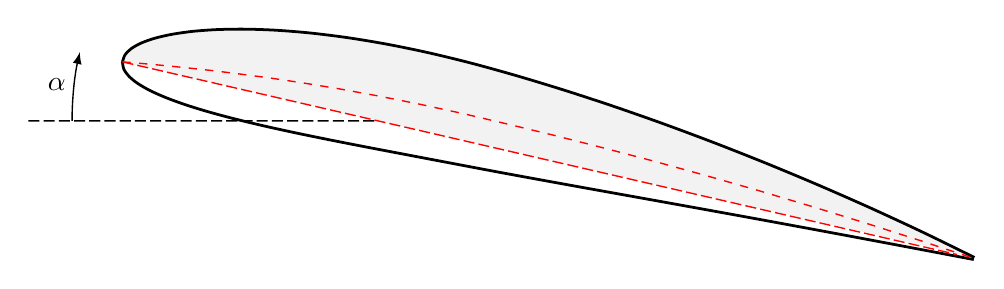
\begin{tikzpicture}[>=latex,scale=1.11]
\tikzstyle{spring}=[snake=zigzag,thick,line before snake=0.3cm,line after  snake=0.3cm,segment length=6,segment amplitude=5,join=round]%
\begin{scope}[rotate around={-13:(10,0)}]
% bottom_second
\draw[smooth,line width=1pt] plot coordinates {(0,0)(0.0334,-0.0767)(0.1087,-0.1437)(0.2253,-0.2011)(0.3824,-0.2489)(0.5790,-0.2870)(0.8139,-0.3158)(1.0860,-0.3355)(1.3940,-0.3466)(1.7365,-0.3497)(2.1123,-0.3457)(2.5199,-0.3356) (2.9580,-0.3209)(3.4252,-0.3029)(3.9198,-0.2835)(4.4427,-0.2625)(4.9936,-0.2377)(5.5666,-0.2102)(6.1594,-0.1810)(6.7696,-0.1513)(7.3950,-0.1217)(8.0332,-0.0930)(8.6815,-0.0653)(9.3376,-0.0386)(9.9988,-0.0125)};
% top_first
\draw[smooth,line width=1pt,fill=black!5] plot coordinates {(0,0)(0.0095,0.0831)(0.0624,0.1691)(0.1590,0.2574)(0.2990,0.3467)(0.4824,0.4357)(0.7085,0.5225)(0.9765,0.6050)(1.2855,0.6812)(1.6341,0.7488)(2.0206,0.8055)(2.4433,0.8492)(2.8998,0.8778)(3.3879,0.8897)(3.9049,0.8833)(4.4459,0.8592)(5.0064,0.8210)(5.5876,0.7687)(6.1870,0.7023)(6.8016,0.6219)(7.4286,0.5277)(8.0650,0.4197)(8.7080,0.2980)(9.3544,0.1623)(10.0012,0.0125)};
% sekelett
\draw[dashed, color=red, line width=0.5pt] plot coordinates { (0.0, 0.0)(0.021, 0.003)(0.086, 0.013)(0.192, 0.028)(0.341, 0.049)(0.531, 0.074)(0.761, 0.103)(1.031, 0.135)(1.34, 0.167)(1.685, 0.2)(2.066, 0.23)(2.482, 0.257)(2.929, 0.278)(3.407, 0.293)(3.912, 0.3)(4.444, 0.298)(5.0, 0.292)(5.577, 0.279)(6.173, 0.261)(6.786, 0.235)(7.412, 0.203)(8.049, 0.163)(8.695, 0.116)(9.346, 0.062)(10.0, 0.0) };
\draw[line width=0.5pt,dashed,dash pattern=on 4pt off 1.5pt,rotate around={13:(3,0)}](-1,0)--(3,0);
% arrows
\draw[line width=0.5pt,<-](3,0) +(180:3.5cm) arc (180:193:3.5cm);
\draw(3,0) +(186.5:3.7cm) node{$\alpha$};
% sehne
\draw[line width=0.5pt,color=red, dashed,dash pattern=on 4pt off 1.5pt](0,0)--(9.8,0);
\end{scope}%
\end{tikzpicture}
\endpgfgraphicnamed%



\begin{tikzpicture}
% profile with data file
%\newcounter{y}
\setcounter{y}{0}
\foreach \x in {1.00}
    \draw (11 cm,1pt) -- (11 cm,-1pt) node[anchor=north] {$\x$};
    \draw (1pt,0 cm) -- (-1pt,0 cm) node[anchor=east] {$0$};
	\draw (1pt,1.25 cm) -- (-1pt,1.25 cm) node[anchor=east] {$0.10$};
	\draw (1pt,-1.25 cm) -- (-1pt,-1.25 cm) node[anchor=east] {$-0.10$};
    \foreach \lbl / \fn in {naca4815.dat}{
        % Some profiles look better when using plot[smooth]
        \draw[yshift=-\arabic{y}cm,scale=11, fill=black!5]% node[left=0.5cm] {\lbl}
            plot file{tikz/data/\fn} -- cycle;
        \stepcounter{y}
    }
% axis
\draw[thick,-] (0,0)  -- (12,0) node[anchor=west] {x};
\draw[thick,-] (0,-2) -- (0,2) node[anchor=south] {y};    
% camber line    
\draw[smooth, dashed, scale=11] plot coordinates {(1.0,0.0)(0.998459,0.000614)(0.993844,0.0024245)(0.986185,0.0053355)(0.975528,0.00919)(0.96194,0.0137755)(0.945503,0.018829)(0.92632,0.0240435)(0.904508,0.029078)(0.880203,0.0335675)(0.853553,0.037132)(0.824724,0.039389)(0.793893,0.0399975)(0.761249,0.0399065)(0.726995,0.039667)(0.691342,0.039262)(0.654508,0.038677)(0.616723,0.037901)(0.578217,0.036926)(0.53923,0.03575)(0.5,0.034375)(0.46077,0.0328075)(0.421783,0.0310595)(0.383277,0.0291465)(0.345492,0.0270885)(0.308658,0.0249115)(0.273005,0.022642)(0.238751,0.0203125)(0.206107,0.0179555)(0.175276,0.0156075)(0.146447,0.013304)(0.119797,0.0110825)(0.095492,0.008979)(0.07368,0.0070285)(0.054497,0.005264)(0.03806,0.0037155)(0.024472,0.0024095)(0.013815,0.0013695)(0.006156,0.000613)(0.001541,0.000154)(0.0,0.0)};    	
\end{tikzpicture}    


\begin{tikzpicture}
% axis
\draw[thick,-] (11,0)  -- (12,0) node[anchor=west] {x};
\draw[thick,-] (0,-2) -- (0,2) node[anchor=south] {y};
% profile with data file
%\newcounter{y}
\setcounter{y}{0}
\foreach \x in {1.00}
    \draw (11 cm,1pt) -- (11 cm,-1pt) node[anchor=north] {$\x$};
    \draw (1pt,0 cm) -- (-1pt,0 cm) node[anchor=east] {$0$};
	\draw (1pt,1.25 cm) -- (-1pt,1.25 cm) node[anchor=east] {$0.10$};
	\draw (1pt,-1.25 cm) -- (-1pt,-1.25 cm) node[anchor=east] {$-0.10$};
    \foreach \lbl / \fn in {naca4815.dat}{
        % Some profiles look better when using plot[smooth]
        \draw[yshift=-\arabic{y}cm,scale=11]% node[left=0.5cm] {\lbl}
            plot file{tikz/data/\fn} -- cycle;
        \stepcounter{y}
    }
% camber line    
\draw[smooth, dashed, color=red, scale=11] plot coordinates {(1.0,0.0)(0.998459,0.000614)(0.993844,0.0024245)(0.986185,0.0053355)(0.975528,0.00919)(0.96194,0.0137755)(0.945503,0.018829)(0.92632,0.0240435)(0.904508,0.029078)(0.880203,0.0335675)(0.853553,0.037132)(0.824724,0.039389)(0.793893,0.0399975)(0.761249,0.0399065)(0.726995,0.039667)(0.691342,0.039262)(0.654508,0.038677)(0.616723,0.037901)(0.578217,0.036926)(0.53923,0.03575)(0.5,0.034375)(0.46077,0.0328075)(0.421783,0.0310595)(0.383277,0.0291465)(0.345492,0.0270885)(0.308658,0.0249115)(0.273005,0.022642)(0.238751,0.0203125)(0.206107,0.0179555)(0.175276,0.0156075)(0.146447,0.013304)(0.119797,0.0110825)(0.095492,0.008979)(0.07368,0.0070285)(0.054497,0.005264)(0.03806,0.0037155)(0.024472,0.0024095)(0.013815,0.0013695)(0.006156,0.000613)(0.001541,0.000154)(0.0,0.0)};  
% sehne
\draw[line width=0.5pt,color=red](0,0)--(11,0);    	
\end{tikzpicture} 
	\caption{Eine Vektorgrafik}
	\label{fig:vectorExample}
\end{figure}










\subsection{Rumpfprofile}
\blindtext






%\newpage
%\newpage\thispagestyle{empty}\hspace{1em}\newpage
\chapter{Eigenes Verfahren}
In diesem Kapitel soll das eigene Verfahren beschrieben werden. Es geht dabei nicht nur darum zu beschreiben was gemacht wurde, sondern ebenfalls darum zu begr�nden, weshalb bestimmte Design-Entscheidungen getroffen wurden.


\section{LaTex-Editoren}

Ein guter Cross-Plattform (Windows/Linux/Mac) Latex-Editor mit englischer und deutscher Rechtschreibkorrektur ist z.B. TexStudio
(\url{http://texstudio.sourceforge.net/}). Unter Windows verwende ich diesen Editor gerne zusammen mit dem Sumatra PDF Viewer (\url{http://blog.kowalczyk.info/software/sumatrapdf/free-pdf-reader.html}), da dieser ein automatisches Neuladen unterst�tzt.

%%%%%%%%%%%%%%%%%%%%%%%%%%%%%%%%%%%%%%%%%%%%%%%%%%%%%%%%%%%%%%%%%%%%%%%%%%%%%%%%%%%%%%%%%%%%%%%%%%%%%%%%%%%%%%%%%%%%%%%%%
\section{Beispiel f�r eine Tabelle}
In Tabelle \ref{tab:bibliotheken} sind die verwendeten Bibliotheken ausgelistet.
\begin{table}[htbp]
\centering 
\begin{tabular}{ll}
\toprule \textbf{Bibliothek} & \textbf{Version} \\
\bottomrule
CUDA SDK & 2.3 \\
CUDA Toolkit & 2.3 \\
 OpenGL & 3.2 \\
 GLUT & 3.7 \\
GLEW & 1.5.1 \\
CUDPP & 1.1 \\
\bottomrule
\end{tabular}
\caption{Die verwendeten Bibliotheken.}
\label{tab:bibliotheken}
\end{table}

\section{Formel in Latex und Konventionen zur Verwendung mathematischer Symbole}
Mathematische Symbole k�nnen in Latex sehr leicht erzeugt werden. Beispiel f�r Symbole im Text: Gegeben sei ein Skalar $a \in \mathbb{R}$. Tabelle~\ref{tab:mathematischeSymbole} liste einige Konventionen zur Verwendung mathematischer Symbole. Abgesetzte Formel lassen sich ebenfalls leicht erzeugen:
\begin{equation}
\label{eqn:beispiel}
f(x) = x^2 + 3
\end{equation}
Au�erdem kann leicht auf abgesetzte Formel verwiesen werden (siehe Gleichung~\ref{eqn:beispiel}). F�r mehrere ausgerichtete Formeln bietet sich die Umgebung \texttt{eqnarray} an:
\begin{eqnarray}
\label{eqn:beispiel2}
f(x) &=& x^2 + 3 \\
g(\theta) &=& \cos (2\theta) = \cos^2 \theta - \sin^2 \theta\\
h(x) &=& \int_0^\infty \mathrm{e}^{-x}\,\mathrm{d}x
\end{eqnarray}


\begin{table}[htbp]
\centering
\begin{tabular}{lll}
\toprule \textbf{Typ} & \textbf{Schriftart} & \textbf{Beispiele} \\
\bottomrule
Variablen (Skalare) & kursiv & $a, b, x, y$ \\
Funktionen & aufrecht& $\mathrm{f}, \mathrm{g}(x), \mathrm{max}(x)$\\
Vektoren & fett, Elemente zeilenweise & $\mathbf{a}, \mathbf{b}= \begin{pmatrix}x\\y\end{pmatrix} = (x, y)^\top$\\
Matrizen & Schreibmaschine& $\mathtt{A}, \mathtt{B}= \begin{bmatrix}a & b\\c & d\end{bmatrix}$\\
Mengen & kalligrafisch& $\mathcal{A}, \{a, b\} \in \mathcal{B}$ \\
Zahlenbereiche & doppelt gestrichen& $\mathbb{N}, \mathbb{Z}, \mathbb{R}^2, \mathbb{R}^3$ \\
\bottomrule
\end{tabular}
\caption{Konventionen zur Verwendung mathematischer Symbole}
\label{tab:mathematischeSymbole}
\end{table}






\section{Beispiel f�r eine Vektorgrafik}

Wenn m�glich sollten immer Vektorgrafiken verwendet werden. Rastergrafiken sollten nur dann eingesetzt werden, wenn die Original-Quelle ebenfalls eine Rastergrafik ist. Ein 
Cross-Plattform Editor zur Erstellung von Vektorgrafiken ist z.B. Inkscape:
\url{http://inkscape.org/download/}. Nach der Erstellung in Inkscape sollte die Grafik zum einen zur sp�teren Weiterverarbeitung als SVG gespeichert werden. Zum anderen zwecks Import in Latex als PDF. Abbildung~\ref{fig:vectorExample} zeigt ein Beispiel.


\begin{figure}[htpb]
	\centering
		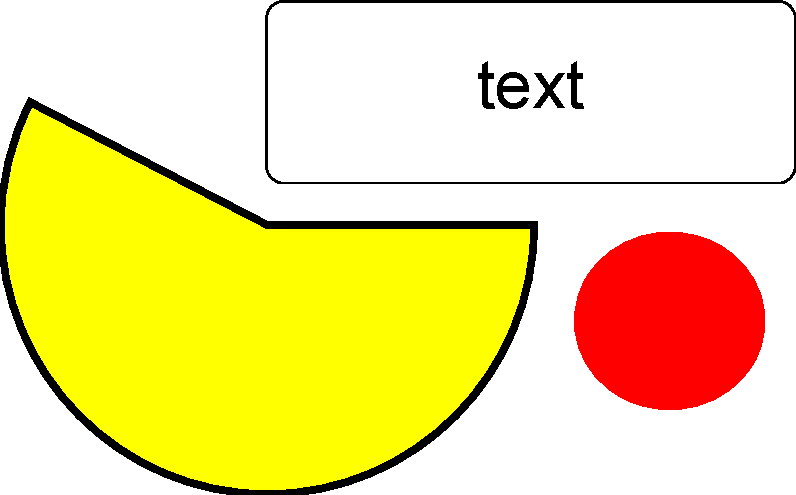
\includegraphics[width=0.30\textwidth]{fig/vectordrawing.pdf}
	\caption{Eine Vektorgrafik}
	\label{fig:vectorExample}
\end{figure}


\section{Beispiel f�r eine Vektorgrafik mit mathematischen Symbolen}

Um beliebigen Latex-Code in eine Vektorgrafik einzuf�gen (z.B. um mathematische Symbole zu setzen) kann in Inkscape beim Speichern der Datei als PDF die Option \glqq Pdf+Latex: Text in PDF weglassen und Latex Datei erstellen\grqq  ~angew�hlt werden (siehe Abb.~\ref{fig:vectorExampleSymbol})

\begin{figure}[htpb]
    \centering
    \def\svgwidth{0.30\textwidth}
  	\import{./fig/}{vectordrawingSymbol.pdf_tex}
	\caption{Eine Vektorgrafik mit mathematischen Symbolen}
	\label{fig:vectorExampleSymbol}
\end{figure}

\section{Beispiel f�r eine Rastergrafik}

Abbildung~\ref{fig:exampleFigure} zeigt, wie eine Rastergrafik eingebunden werden kann. \\

\begin{figure}[htpb]
    \centering
  	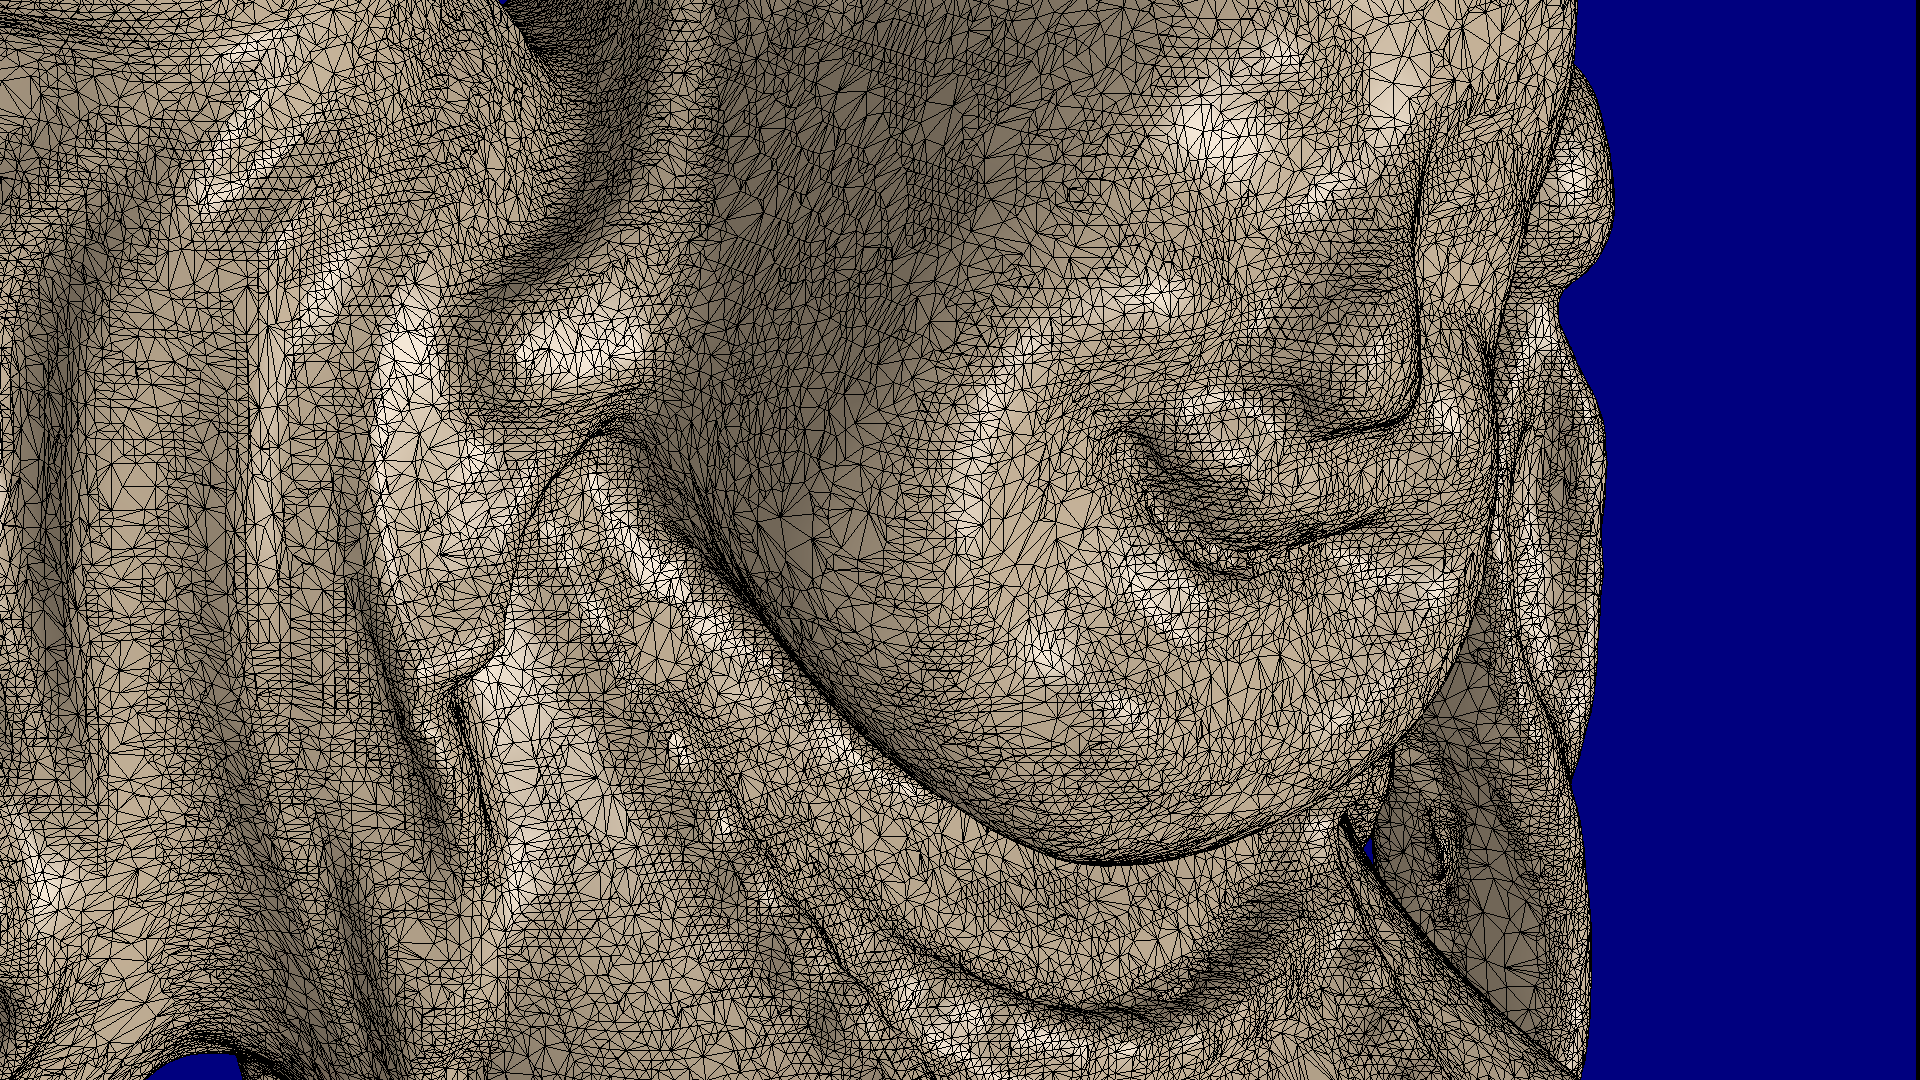
\includegraphics[width=0.80\textwidth]{fig/Buddha2.png}
	\caption{Eine Rastergrafik}
	\label{fig:exampleFigure}
\end{figure}


Bild- bzw. Tabellen-Beschriftungen sollten m�glichst informativ sein. Aus der Beschreibung sollte die Bedeutung der Abbildung vollst�ndig hervorgehen, so dass der Haupttext zum Verst�ndnis nicht notwendigerweise gelesen werden muss. 

\newpage
\section{Beispiel f�r die Darstellung von Algorithmen}

Algorithmus \ref{algo:algorithmSCAN} zeigt ...

\begin{algorithm}[htpb]
	\textit{Phase 1: Reduktion}\\
	\texttt{for} $d := 0$ \texttt{to} $log_2 n - 1$ ~\texttt{in parallel do}\\
	\hspace{5mm}\texttt{for} $k := 0$ \texttt{to} $n - 1$ \texttt{by} $2^{d+1}$ ~\texttt{in parallel do}\\
	\hspace{10mm}$x[k + 2^{d + 1} - 1] := x[k + 2^d - 1] + x [k + 2^{d + 1} - 1]$\\
	\textit{Phase 2: Propagation}\\
	\texttt{for} $d := log_2 n$ \texttt{to} $0$ ~\texttt{in parallel do}\\
	\hspace{5mm}\texttt{for} $k := 0$ \texttt{to} $n - 1$ \texttt{by} $2^{d+1}$ ~\texttt{in parallel do}\\
	\hspace{10mm}$t := x[k + 2^d - 1]$\\
	\hspace{10mm}$x[k + 2^d - 1] := x [k + 2^{d + 1} - 1]$\\
	\hspace{10mm}$x[k + 2^{d + 1} - 1] := t + x [k + 2^{d + 1} - 1]$\\
	\caption{Pseudocode der zwei Phasen vom SCAN-Algorithmus \cite{bib:SCAN}.}
	\label{algo:algorithmSCAN}
\end{algorithm}

\section{Beispiel f�r die Darstellung von Quellcode-Ausz�gen}

dies ist \verb+'+ \LaTeX

Listing \ref{lst:VBOkontrolle} zeigt ...
\lstinputlisting[language=Python, float=htpb, caption={Pseudocode f�r die Kontrolle der VBOs}, label=lst:VBOkontrolle, captionpos=b, keywordstyle=\bfseries\color{black}]{code/test.py}


Listing \ref{lst:VBOkontrolle} zeigt ...
\lstinputlisting[language=Python, style=customc, float=htpb, caption={Pseudocode f�r die Kontrolle der VBOs}, label=lst:VBOkontrolle, captionpos=b, keywordstyle=\bfseries\color{black}]{code/test.py}


Listing \ref{lst:VBOkontrolle} zeigt ...
\lstinputlisting[language=Python, style=customc, float=htpb, caption={Pseudocode f�r die Kontrolle der VBOs}, label=lst:VBOkontrolle, captionpos=b, keywordstyle=\bfseries\color{black}]{code/test2.py}


\section{Hier ein uml diagramm}
\begin{tikzpicture}
\umlemptyclass[width=15ex]{class20}
\umlemptyclass[y=2, width=30ex]{class40}
\end{tikzpicture}


\section{hier kommt pstricks}

\begin{figure}[h]
\centering
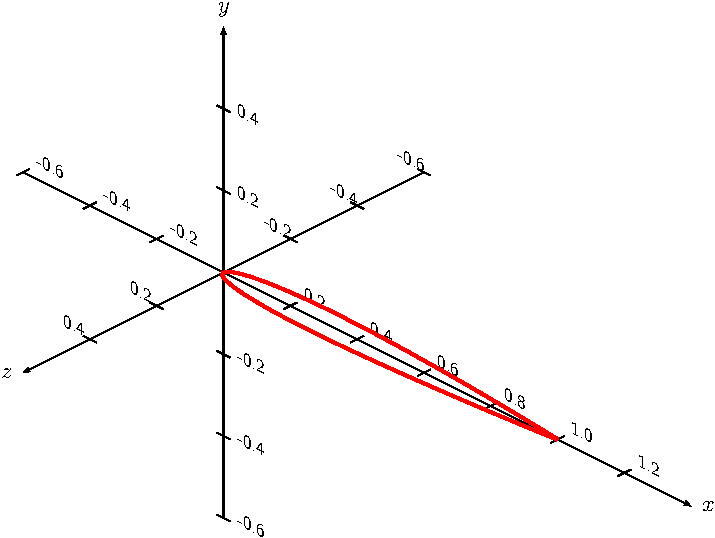
\includegraphics[width=0.7\linewidth]{tikz/Airfoil-crop}
\caption{Mein erster Funktionsplot PSTricks}
\end{figure} %% --> Leerzeile danach wichtig

\begin{figure}[h]
\centering
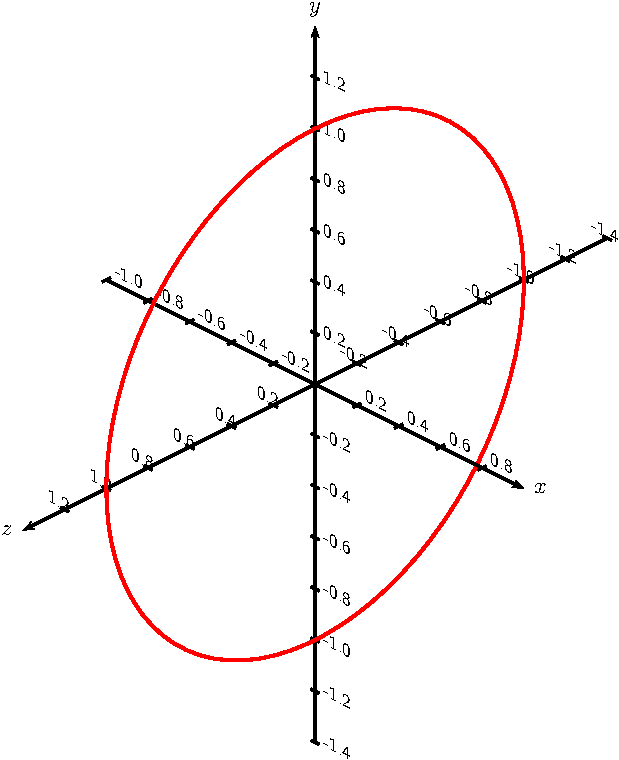
\includegraphics[width=0.7\linewidth]{tikz/Fuselage-crop}
\caption{Mein erster Funktionsplot PSTricks}
\end{figure} %% --> Leerzeile danach wichtig

%\newpage
%\newpage\thispagestyle{empty}\hspace{1em}\newpage
%\chapter{Ergebnisse und Evaluation}
In diesem Kapitel sollen die Ergebnisse dieser Diplomarbeit diskutiert werden. 




%\newpage
%\newpage\thispagestyle{empty}\hspace{1em}\newpage
\chapter{Zusammenfassung und Ausblick}
In diesem Kapitel sollen zun�chst die erreichten Ziele diskutiert und abschlie�end ein Ausblick auf m�gliche, weiterf�hrende Arbeiten gegeben werden.

\newpage
\pagenumbering{Roman}
\setcounter{page}{1}

\nocite{*}%Auch nicht-zitierte BibTeX-Eintr�ge werden angezeigt.
\bibliography{chapters/Literaturverzeichnis}
\bibliographystyle{eg-alpha}
\newpage
\newpage\thispagestyle{empty}\hspace{1em}\newpage
\chapter*{Abk�rzungsverzeichnis}
\begin{acronym}[PM]
 %Sorgt daf�r, dass zwischen den Eintr�gen kein Abstand ist und das Verzeichnis kompakt dargestellt wird.
 \setlength{\itemsep}{-\parsep}
 \acro{ALU}{Arithmetic Logic Unit}
 \acro{BTF}{Bidirektionalen Textur Funktion}
 \acro{CPU}{Central Processing Unit}
 \acro{CU}{Control Unit}
 \acro{CUDA}{Compute Unified Device Architecture}
 \acro{FLOPs}{Floating Point Operations Per Second}
 \acro{FPU}{Floating Point Unit}
 \acro{GPGPU}{General Purpose Compution on Graphics Processing Unit}
 \acro{GPU}{Graphics Processing Unit}
 \acro{HLOD}{Hierarchische Level of Detail}
 \acro{IFS}{Indexed-Face-Set}
 \acro{LOD}{Level of Detail}
 \acro{MIMD}{Multiple Instruction Multiple Data}
 \acro{OpenCL}{Open Computing Language}
 \acro{OpenGL}{Open Graphics Library}
 \acro{PCAM}{Partitionierung Kommunikation Agglomeration Mapping}
 \acro{PM}{Progressive Meshes}
 \acro{SFU}{Spezial Funktion Units}
 \acro{SIMD}{Single Instruction Multiple Data}
 \acro{SIMT}{Single Instruction Multiple Threads}
 \acro{SLI}{Scalable Link Interface}
 \acro{SP}{Streaming-Prozessoren}
 \acro{SM}{Streaming-Multiprozessoren}
 \acro{TPC}{Textur Prozessor Clustern}
 \acro{VBO}{Vertex Buffer Object}

 
\end{acronym}

%Abk�rzungsverzeichnis im Inhaltsverzeichnis anzeigen
\addcontentsline{toc}{chapter}{Abk�rzungsverzeichnis} 
%Abbildungsverzeichnis
\newpage\thispagestyle{empty}\hspace{1em}\newpage
\listoffigures
%Tabellenverzeichnis
\listoftables
%Liste von Algorithmen
\newpage\thispagestyle{empty}\hspace{1em}\newpage
\markboth{Liste der Algorithmen}{Liste der Algorithmen}
\phantomsection
\addcontentsline{toc}{chapter}{Liste der Algorithmen}
\listofalgorithms
%Liste von Code
\newpage\thispagestyle{empty}\hspace{1em}\newpage
\markboth{Listings}{Listings}
\phantomsection
\addcontentsline{toc}{chapter}{Listings}
\lstlistoflistings
%Anhang
\newpage
\newpage\thispagestyle{empty}\hspace{1em}\newpage
\appendix
\chapter{Anhang}\label{chp:AnhangA}
\section*{Thema 1}\label{sec:AnhangA1}

Beispiel f�r einen Anhang

\section*{Thema 2}\label{sec:AnhangA2}

%Danksagung
\chapter*{Danksagung}
Hiermit m�chte ich mich besonders bei Prof. Dr. XXXX, Prof. Dr. xxxx, Dipl. Inf. xxxx und Dipl. Inf. xxx f�r die Betreuung meiner Arbeit, hilfreiche Diskussionen und viel Geduld bei zahlreichen Fragen bedanken.
\end{document} "
\end{codeexample}
\noindent where |main-figure0| is the picture we are currently externalizing and |main.tex| is the main document.

As soon as ``conversion mode'' has been detected, \pgfname\ changes the output routine. The complete file |main.tex| is processed as normal, but only the part of the desired picture will be written to the output file, in our case |main-figure0.pdf|. The rest of the document is silently thrown away. Of course, such a conversion process is quite expensive since we need to do it for every picture. Since everything except the current picture is thrown away, the library skips all other pictures. Furthermore, any |\includegraphics| commands which are outside of the converted \tikzname-picture will be skipped as well. Thus, the conversion process should be much faster than typesetting the complete document, but it still requires its time.
Eventually, the call |% das Papierformat zuerst
%
%\documentclass[a4paper, 11pt,bibtotoc]{scrartcl}
\documentclass[a4paper, 12pt, oneside, final, bibtotoc,abstracton]{scrreprt}  

%\documentclass[
%	a4paper,
%	12pt,
%	oneside,
%	%twoside,
%	%openright,
%	final
%	%draft,				% Entwurf: Druckt keine Bilder
%]{scrreprt}


%F�r URL
\usepackage{url}
\renewcommand{\UrlFont}{\rmfamily}

%F�r Zitaten
\usepackage{cite}

%Abk�rzungen
\usepackage{acronym}


%Inhaltsverzeichnis bearbeiten
\usepackage{tocbibind}

% f�r mathematische Symbole
\usepackage{amsmath}

% tabellen
\usepackage{tabularx}

% Vektorgrafiken mit Latex importieren
\usepackage{import}

\usepackage[colorlinks=false, pdfborder={0 0 0}]{hyperref}
%documentclass[a4paper, 12pt]{article}  
% deutsche Silbentrennung
\usepackage[english,ngerman]{babel}
\renewcommand{\sectfont}{\rmfamily\bfseries}
% wegen deutschen Umlauten
\usepackage[ansinew]{inputenc}
\usepackage{graphicx}
\usepackage{subfigure}\hyphenation{Bit-rate}

%Algorithm schreiben
\usepackage{algorithm2e}

%Tabellen
\usepackage{booktabs}
\usepackage{multirow}
\usepackage{colortbl}


%Farben
\usepackage{xcolor}
\usepackage{color}
\usepackage{listings}%Code einbinden
\definecolor{darkblue}{rgb}{.08,.21,.36}
\definecolor{darkred}{rgb}{.6,.19,.20}
\definecolor{darkgreen}{rgb}{0,.6,0}
\definecolor{red}{rgb}{.98,0,0}
\definecolor{lightblue}{rgb}{0.8,0.85,1}
%\definecolor{lightgrey}{rgb}{0.98,0.98,0.98}
\definecolor{lightgrey}{gray}{.98}
\definecolor{black}{rgb}{0.0,0.0,0.0}


\lstloadlanguages{C++}
\lstset{%
  language=Python,
  basicstyle=\small,
  commentstyle=\itshape\color{darkgreen},
  keywordstyle=\bfseries\color{darkblue},
  stringstyle=\color{darkred},
  showspaces=false,
  showtabs=false,
  columns=fixed,
  backgroundcolor=\color{lightgrey},
  numbers=left,
  frame=single,
  numberstyle=\tiny,
  breaklines=true,
  showstringspaces=false,
  xleftmargin=1cm,
  basicstyle=\small
}%

\usepackage{amssymb}%Mathematische Symbole, wie R,N,Q,Z,...
\setlength{\parindent}{0pt} %einr�cken nach absatz verhindern
%\usepackage{setspace}%Zeilenabstand
\usepackage{algorithmic}%F�r Pseudocode

%%%%%%%%%%%%%%%%%%%%%%%%%%%%%%%%%%%
%Seiten Kopf- und Fu�zeilen
\usepackage[automark,						
		headsepline,								
		plainfootsepline, 
		]{scrpage2}

\automark[section]{chapter} 
\pagestyle{scrheadings}			

\clearscrheadings	%Alte Kopfformatierungen entfernen
\clearscrplain		%Alte Plain-Formatierung entfernen
\clearscrheadfoot %Alten Fu� entfernen
\cfoot[\pagemark]{\pagemark}%Seitenzahl zentriert im Fu� 
\ihead{\leftmark}
\ohead{\rightmark} 


%%%%%%%%%%%%%%%%%%%%%%%%%%%%%% User specified LaTeX commands.

% Mehr Platz zwischen Tabelle und Untertitel
\usepackage{caption}
\captionsetup[table]{skip=10pt}


\colorlet{chapter}{black!75}
\addtokomafont{chapter}{\color{chapter}}
%

%Kapitelzahl sehr gro�
\makeatletter% siehe De-TeX-FAQ 
 \renewcommand*{\chapterformat}{% 
   \begingroup% damit \unitlength-�nderung lokal bleibt 
     \setlength{\unitlength}{1mm}% 
     \begin{picture}(10,10)(0,5) 
       \setlength{\fboxsep}{0pt} 
       %\put(0,0){\framebox(20,40){}}% 
       %\put(0,20){\makebox(20,20){\rule{20\unitlength}{20\unitlength}}}% 
       \put(10,15){\line(1,0){\dimexpr 
           \textwidth-20\unitlength\relax\@gobble}}% 
       \put(0,0){\makebox(10,20)[r]{% 
           \fontsize{28\unitlength}{28\unitlength}\selectfont\thechapter 
           \kern-.05em% Ziffer in der Zeichenzelle nach rechts schieben 
         }}% 
       \put(10,15){\makebox(\dimexpr 
           \textwidth-20\unitlength\relax\@gobble,\ht\strutbox\@gobble)[l]{% 
             \ \normalsize\color{black}\chapapp~\thechapter\autodot 
           }}% 
     \end{picture} % <-- Leerzeichen ist hier beabsichtigt! 
   \endgroup 
}
\makeatother% siehe \makeatletter

\usepackage{ %a4wide,
            ellipsis, fixltx2e, mparhack,   %Fehlerkorrektur f�r Marginalien
            booktabs, longtable             %sch�nere Tabellen
}  

\usepackage{ifpdf} % part of the hyperref bundle
\ifpdf % if pdflatex is used


%set fonts for nicer pdf view
 \IfFileExists{lmodern.sty}{\usepackage{lmodern}}
  {\usepackage[scaled=0.92]{helvet}
    \usepackage{mathptmx}
    \usepackage{courier} }
\fi

%%%%%%%%%%%%%%%%%%%%%%%%%%%%%%%%%%%%%%%%%%%%%%%%%%%%%%%%%%

% sch�nerer Blocksatz!!
\usepackage{microtype}
 
%%%%%%%%%%%%%%%%%%%%%%%%%%%%%%%%%%%

% Hurenkinder und Schusterjungen werden vermieden
\clubpenalty = 10000
\widowpenalty = 10000
\displaywidowpenalty = 10000

%%%%%%%%%%%%%%%%%%%%%%%%%%%%%%%%%%%%%%%%%%%%%%%%%%%%%%%%%%%%%%%%%%%%%
%%% Definitionen
%%%%%%%%%%%%%%%%%%%%%%%%%%%%%%%%%%%%%%%%%%%%%%%%%%%%%%%%%%%%%%%%%%%%%
\begin{filecontents}{cpuAnno.dat}
0 0 5 0.8 20 13.3 35 19.6 50 0.3
\end{filecontents} 
%%%%%%%%%%%%%%%%%%%%%%%%%%%%%%%%%%%%%%%%%%%%%%%%%%%%%%%%%%%%%%%%%%%%%
%%% End Definitionen
%%%%%%%%%%%%%%%%%%%%%%%%%%%%%%%%%%%%%%%%%%%%%%%%%%%%%%%%%%%%%%%%%%%%%


\begin{document}
%\begin{titlepage}
%\begin{center}
%{\huge \textbf{Philipps-Universit�t Marburg}}\\[0.5cm]
%\textbf{Fachbereich 12 - Mathematik und Informatik}\\[0.5cm]
%
%\begin{figure}[h]
%	\centering
%		
\includegraphics[width=0.8\textwidth]{fig/unilogo.pdf}
%\end{figure}
%
%{\huge \textbf{{\large \\[1cm]Masterarbeit}}}
%\\[1cm]
%
%{\huge \textbf{Entwicklung eines interaktiven Editors f�r Flugzeugkonfigurationen ~~~~~~~~~~~~~~ im Vorentwurf}}
%\\[1cm]
%
%{\large von}\\
%{\large Ren\'{e} Frank}\\
%{\large Januar 2015}\\[1.5cm]
%
%{\large
%Betreuer:\\Prof. Dr. Thorsten Thorm�hlen\\[0.5cm]
%Arbeitsgruppe Grafik und Multimedia Programmierung}
%\\[0.8cm]
%{\large
%Betreuer:\\Carsten Liersch\\[0.5cm]Deutsches Zentrum f�r Luft- und Raumfahrt (DLR)\\
%Institut f�r Aerodynamik und Str�mungstechnik}
%
%
%
%
%
%
%
%\end{center}
%\end{titlepage}

%\setstretch {1.15}%Zeilenabstand setzen

  
% hier beginnt das Dokument
\begin{titlepage}
	
\vspace{0.3cm} \noindent\rule{\textwidth}{0.5mm} \vspace{-0.3cm}	
	
%\begin{minipage}{19mm} 
%    %
\includegraphics{fig/siegel_uni.pdf}
%    
\includegraphics{fig/siegel-philipp.eps}
%        
\includegraphics[width=\linewidth]{fig/DLR_Logo.eps}
%\end{minipage}
%	\hfill	
%\begin{minipage}{85mm}	
%	\sffamily
%	%\noindent\Large\textbf{\input{graphics/siegel-philipp.eps}}  
%	
%\begin{flushright}
%	\scriptsize FACHBEREICH MATHEMATIK UND INFORMATIK
%
%	\vspace{0.25cm}
%	
%	\scriptsize Arbeitsgruppe Grafik und Multimedia Programmierung
%\end{flushright}
%
%\end{minipage}	


\begin{minipage}{\linewidth} 
    
\includegraphics{fig/siegel-philipp.eps}
	\hfill	 
    
\includegraphics[scale=0.15]{fig/DLR_Logo}
\end{minipage}

\begin{minipage}{\linewidth}	
	\sffamily
	%\noindent\Large\textbf{\input{graphics/siegel-philipp.eps}}  	
\begin{flushleft}
	\vspace{0.25cm}
		
	\scriptsize FACHBEREICH MATHEMATIK UND INFORMATIK %\hfill Institut f�r Aerodynamik und Str�mungstechnik% DEUTSCHES ZENTRUM F\"UR LUFT- UND RAUMFAHRT%Deutsches Zentrum f�r Luft- und Raumfahrt
	
	\vspace{0.25cm}	

	\scriptsize Arbeitsgruppe Grafik und Multimedia Programmierung \hfill Institut f�r Aerodynamik und Str�mungstechnik 
\end{flushleft}

\end{minipage}	
 
	
%	\noindent\footnotesize Philipps-Universit\"at Marburg,\\
%	\footnotesize Fachbereich 12: Mathematik und Informatik \hfill \today
	\vspace{0.3cm} \noindent\rule{\textwidth}{0.1mm}\vspace{1cm}
	\rmfamily\normalsize	



\begin{center}
\Large{\textsf{\textbf{Entwicklung eines interaktiven Editors f\"ur Flugzeugkonfigurationen im Vorentwurf}}}
 
\vspace{1em}
 
\large{\textsf{Abschlussarbeit zur Erlangung des akademischen Grades}} \\
\Large{\textsf{Master of Science (M.Sc.)}} \\
\large{\textsf{vorgelegt von}}
 
\vspace{0.5em}
 
\textsf{Ren\'{e} Frank B.Sc.}
 
\vspace{5.0em}
 
%\textsf{\makebox[3.5cm][l]{Referentin:}}            \textsf{\makebox[7cm][r]{Prof. Dr. ...}} \\
\textsf{\makebox[3.5cm][l]{Betreuer:}}           \textsf{\makebox[7cm][r]{Prof. Dr. Thorsten Thorm\"ahlen
}} \\
\textsf{\makebox[3.5cm][l]{Betreuer:}}           \textsf{\makebox[7cm][r]{Dipl.-Ing. Carsten Liersch
}}
 

 
 
\textsf{\small{\makebox[3.5cm][l]{Ausgabedatum:}}}  %\textsf{\small{\makebox[7cm][r]{24.05.2012}}}
\textsf{\small{\makebox[7cm][r]{XX.XX.2014}}} \\
 
\textsf{\small{\makebox[3.5cm][l]{Abgabedatum:}}}   %\textsf{\small{\makebox[7cm][r]{01.10.2012}}}
\textsf{\small{\makebox[7cm][r]{XX.XX.2015}}}
\vfill
%\vspace{2cm}


Philipps-Universit\"at Marburg\\
Fachbereich Mathematik und Informatik\\
Hans-Meerwein-Stra\ss e\\
35032 Marburg

\end{center}

\end{titlepage}

\newpage
\shipout\null
\chapter*{Erkl\"arung}
\thispagestyle{empty}

\normalsize
Ich erkl\"are hiermit, dass ich diese Masterarbeit mit dem Titel \textit{Entwicklung eines interaktiven Editors f\"ur Flugzeugkonfigurationen im Vorentwurf} selbstst\"andig ohne Hilfe Dritter und ohne Benutzung anderer als der angegebenen Quellen und Hilfsmittel verfasst habe. Alle den benutzten Quellen w\"ortlich oder sinngem\"a\ss {} entnommenen Stellen sind als solche einzeln kenntlich gemacht.\\

\noindent Diese Arbeit ist bislang keiner anderen Pr\"ufungsbeh\"orde vorgelegt und auch nicht ver\"offentlicht worden.\\

\noindent Ich bin mir bewusst, dass eine falsche Erkl\"arung rechtliche Folgen haben wird.\\[3cm]

 
\vspace{5em}
 
\begin{flushright}
\begin{table}[ht]
\begin{tabularx}{\textwidth}{Xp{7cm}}
%Marburg den \today & \tabularnewline \cline{2-2}  \addlinespace
Marburg den 13.08.12 & \tabularnewline \cline{2-2}  \addlinespace
 & \centering{Ren\'{e} Frank}
\end{tabularx}
\end{table}
\end{flushright}

\begin{abstract}
Viele der in der Computergrafik verwendeten 3D-Modelle werden mit Hilfe der Dreiecksnetze  repr�sentiert. ... (max. 1 Seite)
\end{abstract}

\begin{otherlanguage}{english}
\begin{abstract}
text text text text text text
text text text text
text text text text text text text texttext text
(exakte englische �bersetzung der deutschen Kurzfassung)
\end{abstract}
\end{otherlanguage} 

\newpage
\thispagestyle{empty}
%% Ab jetzt r�mische Seitenzahlen
\pagenumbering{Roman}
\setcounter{page}{0}
\hspace{1cm}
\tableofcontents
\newpage
\pagenumbering{arabic}
\setcounter{page}{1}
\chapter{Einleitung}
Diese Diplomarbeit besch�ftigt sich mit den Parallel View-Dependent Compressed Progressive Meshes und deren Umsetzung in die vom Grafikkartenhersteller NVIDIA entwickelte parallele Programmiersprache CUDA. Dazu geh�rt die Entwicklung einer f�r die parallele Verarbeitung geeignete effiziente Datenstruktur, sowie eine effiziente Datenverwaltung.  

%%%%%%%%%%%%%%%%%%%%%%%%%%%%%%%%%%%%%%%%%%%%%%%%%%%%%%%%%%%%%%%%%%%%%%%%%%%%%%%%%%%
\section{Motivation}
Die aktuelle Entwicklung der Multimediaindustrie versucht zunehmend die Simulation von virtuellen Welten realistisch darzustellen. Die Anspr�che der Anwender werden mit der Zeit immer gr��er und dementsprechend die generierte virtuelle Realit�t immer komplexer. So eine Entwicklung ist unweigerlich mit der  Steigerung der erforderlichen Rechenleistung verbunden, da die simulierten Objekte aus  Millionen von Polygonen bestehen k�nnen und  in Echtzeit dargestellt werden m�ssen.
Im Laufe der Jahre sind viele verschiedene Verfahren entwickelt worden, die das Ziel hatten, die komplexen Objekte mit einem vertretbaren Qualit�tsverlust in Echtzeit darzustellen. Der mit Abstand beste Ansatz, um den Kompromiss zwischen Qualit�t und Geschwindigkeit zu finden, ist die View-Dependent Progressive Meshes. Einer der Vorteile dieser Herangehensweise ist, dass dieses Verfahren hochgradig parallelisierbar ist, so dass sich mit einer geeigneter Programmiersprache und Hardware eine beachtliche Effizienzsteigerung erzielen l�sst.\\
Die von NVIDIA entwickelte parallele Programmiersprache CUDA setzt auf den aktuellen Trend der GPGPUs und  erm�glicht es mit einer kosteng�nstigen Grafikkarte, die in fast jeden Desktoprechner vorhanden ist, Programme effizient zu parallelisieren. Aus diesem Grund ist CUDA f�r das Parallelisieren von View-Dependent Progressive Meshing besonders geeignet.

%%%%%%%%%%%%%%%%%%%%%%%%%%%%%%%%%%%%%%%%%%%%%%%%%%%%%%%%%%%%%%%%%%%%%%%%%%%%%%%%%%%
\section{Ziele}\label{chp:Ziele}   
Das Ziel dieser Arbeit ist die Entwicklung einer effizienten parallelen Implementierung  von komprimierten View-Dependent Progressive Meshes in CUDA, welche in der Lage ist, Objekte die aus mehreren Millionen von Polygonen bestehen k�nnen, in Echtzeit zu verarbeiten.

%%%%%%%%%%%%%
\subsubsection{Echtzeit} 
Das entwickelte Programm soll selbst sehr gro�e Polygonnetze effizient verarbeiten k�nnen. Die Eingaben des Benutzers f�r die Translation und Rotation des Objekts sollen in Echtzeit umgesetzt werden. Die durchschnittliche Laufzeit des Programms pro Frame soll h�chstens drei Mal soviel Zeit wie das Rendering des gegebenen Modells ben�tigen, um eine Echtzeitdarstellung des Modells zu erm�glichen. Dabei k�nnen die Modelle aus mehreren Millionen von Dreiecken bestehen.

%%%%%%%%%%%%%
\subsubsection{Kosten} 
Das Programm sollte mit der normalen, kosteng�nstigen Privatanwender-Hardware laufen, sodass f�r die Ausf�hrung keine Spezialrechner ben�tigt werden. Die einzige Vorrausetzung an das System ist eine NVIDIA-Grafikkarte die CUDA 1.1 unterst�tzt. Diese ist aber in den meisten Desktoprechnern vorhanden oder kann kosteng�nstig nachger�stet werden. 

%%%%%%%%%%%%%%%%%%%%%%%%%%%%%%%%%%%%%%%%%%%%%%%%%%%%%%%%%%%%%%%%%%%%%%%%%%%%%%%%%%%
\section{Aufbau der Arbeit}
Im ersten Abschnitt des Kapitels~\ref{chp:CUDA} soll zun�chst die Bedeutung der Grafikkarte als Berechnungseinheit verdeutlicht werden. Dann soll  im zweiten Abschnitt die Hard- und Softwarearchitektur der Programmiersprache \acs{CUDA} beschrieben werden, sowie einige Vorschl�ge zu Codeoptimierung diskutiert, bevor im Kapitel~\ref{chp:ProgressiveMeshes} ein �berblick �ber die wichtigsten Verfahren zur Echtzeitdarstellung komplexer Objekte geben wird. An dieser Stelle werden auch das View-Dependent Progressive Meshing, sowie einige Simplifizierungstechniken genauer erl�utern.        Kapitel~\ref{chp:ParallelViewDependentRefinementofComprPM} besch�ftigt sich mit der Theorie des im Rahmen dieser Diplomarbeit entwickelten Algorithmus. Dabei sollen die Datenstrukturen, die Kompression, sowie die einzelnen Schritte des Algorithmus genauer erl�utert werden. Die Implementierung des Algorithmus in \acs{CUDA} wird im Kapitel 5 besprochen, dabei sollen die benutzten Bibliotheken, sowie die \acs{CUDA}-spezifische Umsetzung des Programms beschrieben werden. Anschlie�end werden im Kapitel 6 die durchgef�hrten Tests und deren Ergebnisse dokumentiert und diskutiert, sowie im Kapitel 7 ein Ausblick auf weiterf�hrende Arbeiten gegeben. 


%%%%%%%%%%%%%%%%%%%%%%%%%%%%%%%%%%%%%%%%%%%%%%%%%%%%%%%%%%%%%%%%%%%%%%%%%%%%%%%%%%%
\section{Verwandte Arbeiten}
Im  Themenbereich der Progressive Meshes und View-Dependent Progressive Meshes gab es schon am Ende des letzten Jahrzehnts einige  Ver�ffentlichungen \cite{bib:hoppePM, bib:hoppeVPM}.  Diese waren zwar eine gute und notwendige Weiterentwicklung vom klassischen LOD-Algorithmus, erm�glichten aber nicht eine effiziente Echtzeitdarstellung von gro�en Modellen. In \cite{bib:efPM} wurde schlie�lich ein Versuch unternommen eine effizientere Datenstrucktur zu entwickeln, um den Speicherverbrauch zu optimieren und bessere Geschwindigkeit zu erreichen. Diese effizientere Datenstruktur brachte zwar einige Verbesserungen, erm�glichte aber dennoch keine  Echtzeitdarstellung von gro�en Modellen. 
Seit dem gab es eine Reihe von Verfahren, die das Ziel hatten eine effiziente Echtzeitdarstellung von gro�en Modellen zu erm�glichen. Einige von diesen Verfahren nutzten Multi-Triangulationen \cite{bib:DFMP98}, andere Versuchten die  View-Dependent Progressive Meshes weiterzuentwickeln \cite{bib:PAJ01, bib:PD04 ,bib:ESV99}. Doch keins dieser Verfahren konnte die Anforderungen vollst�ndig erf�llen.\\
Eine erst k�rzlich ver�ffentlichte Arbeit \cite{bib:Hoppe2009} machte endlich einen Schritt in die richtige Richtung. Die in dieser Arbeit implementierte GPU-Variante von  parallelen View-Dependent Progressive Meshes erm�glichte eine akzeptable Echtzeitdarstellung von gro�en Modellen. Diese braucht durchschnittlich das dreifache der Zeit, die f�r das Rendering des  Modells ben�tigen wird und l�sst somit einen gro�en Spielraum f�r die Optimierung offen.  

 

%\newpage
%\newpage\thispagestyle{empty}\hspace{1em}\newpage
%\chapter{Grundlagen}\label{chp:Grundlagen}
Im Folgenden soll ein \"Uberblick über die in dieser Arbeit verwendeten Technologien gegeben
werden. Eine allgemeine Einf\"uhrung in den Flugzeugentwurfsprozess zeigt anfangs die Einsatzgebiete des SGG-Editors auf.
Weiterhin wird auf das zentrale Datenformat CPACS, auf dem der SGG arbeitet, eingegangen und dessen Aufbau erl\"autert.
Im zweiten Teil werden die dargestellten Flugzeugkomponenten und verwendete Generierungsverfahren vorgestellt.

\section{Flugzeugentwurf}\label{sec:CPACS}
hier steht alles zum Flugzeugentwurfsprozess

\section{CPACS}\label{sec:CPACS}
Wie schon in Kapitel~\ref{sec:CPACS} beschrieben ... steht hier alles zu CPACS

\section{Profile}
Die Form des Querschnitts eines K\"orpers, wird im Folgenden als Profil bezeichnet. In der Aerodynamik ist die Entwicklung und Charakterisierung von Profilen ein wichtiges Teilgebiet. Konstruierte Profile sollen in ihrer Form bestimmten Funktionen gen\"ugen wie beispielsweise die Erzeugung eines dynamischem Auftriebs bei geringem Strömungswiderstand. In Cpacs wird zwischen Rumpf- und Tragfl\"achenprofilen unterschieden. Beide Profiltypen sind unter dem Konten \textit{profiles} als Listen f\"ur x, y und z Koordinaten repr\"asentiert.\\\\

	ooo hier steht ein tikz xml editor\\\\ 

\subsection{Fl\"ugelprofile}
hier steht allgemeines Zeug zu den Profilen

\newcounter{y}
\setcounter{y}{0}

\begin{tikzpicture}
    \foreach \lbl / \fn in {EPPLER 625/e625.dat,
                            WORTMANN FX 2/fx2.dat,
                            EPPLER 664 (EXTENDED)/e664ex.dat,
                            CLARK Y/clarcy.dat,
                            Eiffel 10 (Wright)/eiffel10.dat,
                            FX 69-PR-281/fx69pr281.dat,
                            NACA Munk M-4 airfoil/m4.dat}{
        % Some profiles look better when using plot[smooth]
        \draw[yshift=-\arabic{y}cm,scale=3] node[left=0.5cm] {\lbl}
            plot file{tikz/data/\fn} -- cycle;
        \stepcounter{y}
    }  
\end{tikzpicture}
\footnotetext{Quelle: http://www.texample.net/tikz/examples/airfoil-profiles, Zugriff: 27.10.2014}


\subsubsection{NACA-Serie}
Das National Advisory Committee for Aeronautics oder kurz NACA wurde 1915 gegründet und ist ein direkter Vorg\"anger der US-Bundesbehörde für Luft- und Raumfahrt, NASA. Die NACA war eine amerikanische Organisation, die sich mit der Grundlagenforschung in der Luftfahrt beschäftigte. Eine bedeutende Entwicklung der NACA-Forschungen, sind optimierte Tragf\"achenprofile. Durch aerodynamischen Tests im Windkanal wurde bereits fr\"uh erkannt, dass die Fl\"ugelprofile mit den besten Eigenschaften hinsichtlich Auftriebsbeiwert und Widerstandsbeiwert, viele Gemeinsamkeiten besitzen. NACA-Profile sind somit Variationen eines Ursprungsprofils, die mit Hilfe von analytischen Gleichungen definiert werden. Spezifische Variationen dieses Profils werden durch die Kr\"ummung bzw. Steigung der Skelettlinie sowie die Dicke der Tragfl\"ache oberhalb und unterhalb jener Skelettlinie erzeugt. Im SGG-Editor wurde ein NACA-Generator implementiert, mit dem sich Profile der NACA 4-digit und NACA 5-digit Serie erstellen lassen.

\paragraph{Profile der Vierer-Serie}

In der vierstelligen NACA-Serie ist ein Profil definiert durch:
\begin{itemize}
\item[1.]Ziffer: maximale Profilw\"olbung 
	\begin{itemize}
		\item angegeben in Prozent, bezogen auf die L\"ange der Profilsehne
	\end{itemize}
\item[2.]Ziffer: W\"olbungsrücklage, Position der maximalen Profilw\"olbung
	\begin{itemize}
		\item angegeben in Zehnteln der L\"ange der Profilsehne
	\end{itemize}
\item[3./4.]Ziffer: maximale Profildicke
	\begin{itemize}
		\item angegeben in Prozent, bezogen auf die L\"ange der Profilsehne
	\end{itemize}
\end{itemize} 


Ein symmetrisches NACA 4 Profil kann mit Gleichung \ref{eq:symyt} konstruiert werden. Das Profil ist in seiner Form, nur durch die angegebene Profildicke ver\"andertbar, da die Profilw\"olbung und somit auch dessen Position die Werte Null haben. Gleichung \ref{eq:symyt} enth\"alt Konstanten, die f\"ur eine Profildicke von 20\% vorgesehen sind. Um diese Werte an die jeweils angegebene Profildicke anzupassen, wird die eigentliche Berechung mit $\frac{t}{0.2}$ multipliziert. In Gleichung \ref{eq:symyt} werden zus\"atzlich folgende Parameter verwendet:

\begin{itemize}
	\item[$c$ :] L\"ange der Profilsehne
	\item[$x$ :] Position entlang der Profilsehne auf der Abszissenachse von 0 to c, 
	\item[$y_t$ :] Entfernung der Skelettlinie zur jeweiligen Profilseite an Position x
	\item[$t$ :] Maximale Dicke des Profils multipliziert mit $\frac{1}{100}$
\end{itemize}

\begin{multline}\label{eq:symyt}
y_t= \frac{t}{0.2}c\left[0.2969 \sqrt{\frac{x}{c}} + (-0.1260) \left(\frac{x}{c}\right) + (-0.3516) \left(\frac{x}{c}\right)^2 + 0.2842 \left(\frac{x}{c}\right)^3 \right. \\\left. + (-1.015) \left(\frac{x}{c}\right)^4 \right]
\end{multline}


Soll die trailing edge geschlossen sein, also das Profil an dieser Position eine Dicke gleich Null haben, wird als Koeffizient an der letzen Stelle statt $-1.015$ ein Wert von $-0.1036$ gew\"ahlt.  Es ergeben sich folgende Definitionen f\"ur Ober- und Unterseite des Profils. Die x-Koordinaten sind f\"ur beide Seiten gleich, daher gilt $x_U = x_L = x$. Die y-Koordinaten ebenfalls identisch, nur das diese f\"ur die Oberseite positiv: $y_U = +y_t$ und f\"ur die Unterseite negativ sind: $y_L = -y_t$.\\
Die Generierung eines asymmetrischen NACA 4 Profils braucht zus\"atzlich zu Gleichung \ref{eq:symyt} noch die maximale Profilw\"olbung und die W\"olbungsr\"ucklage, also den Abstand der Profilnase zur maximalen Profilw\"olbung. 

\begin{itemize}
	\item[$m$ :] Maximale W\"olbung multipliziert mit $\frac{1}{100}$
	\item[$p$ :] Position der maximalen W\"olbung multipliziert mit $\frac{1}{10}$ 
	\item[$t$ :] Maximale Dicke des Profils multipliziert mit $\frac{1}{100}$	
\end{itemize}

Mit Gleichung \ref{eq:camber} wird die y-Koordinate der Skelettlinie an einer gegebenen x-Koordinate berechnet. 

\begin{equation}\label{eq:camber}
     y_c = \left\{ \begin{array}{ll} 
     					m \frac{x}{p^2} \left(2p - \frac{x}{c}\right), & 0 \leq x \leq pc \\[0.5cm]
         				m \frac{c-x}{(1-p)^2}\left(1+\frac{x}{c}-2p\right), & pc \leq x \leq c
         			\end{array}\right.
\end{equation}

\vspace{0.5cm}
Die Dicke des gekr\"ummten Fl\"ugelprofils ist senkrecht zur Skelettlinie festgelegt womit f�r Ober- und Unterseite des Profils folgendes gilt:

\begin{equation}
x_U = x - y_t \sin \theta \qquad , \qquad y_U = y_c + y_t \cos \theta
\end{equation}
\begin{equation}
x_L = x + y_t \sin \theta \qquad , \qquad y_L = y_c +-y_t \cos \theta
\end{equation}


$\theta = \arctan \left(\frac{dy_c}{dx}\right)$

\begin{equation}\label{eq:camber}
     \frac{dy_c}{dx} = \left\{ \begin{array}{ll} 
     					\frac{2m}{p^2} \left(p - \frac{x}{c}\right), & 0 \leq x \leq pc \\[0.5cm]
         				\frac{2m}{(1-p)^2}\left(p - \frac{x}{c}\right), & pc \leq x \leq c
         			\end{array}\right.
\end{equation}



text \cite{bib:naca_docu}
\subsubsection{Naca5}

Um den maximalen Auftrieb von Tragfl\"achenprofilen zu erh\"ohen, wurde zus\"atzlich die 5er Naca Serie entwickelt. Ein NACA 5 Profil hat die Form LPQXX (beispielsweise NACA 23009) und wird wie im Folgenden definiert. Hierbei ist zu beachten, dass die ersten beiden Ziffern zur sp\"ateren Berechnung umgrechnet werden.

\begin{enumerate}
	\item Ziffer: Wert zur Berechnung des optimalen Auftriebskoeffizienten bei optimalem Anstellwinkel
		\begin{itemize}
			\item $cl = L * 0.15 $
		\end{itemize}	
	\item Ziffer: Position der gr\"o\ss ten W\"olbung entlang der Sehnenlinie, beginnend bei der leading edge
		\begin{itemize}
			\item $p = P * 5 $
		\end{itemize}
	\item Ziffer: einfache oder gespiegelte Kr\"ummung
		\begin{itemize}
			\item $0$ oder $1$
		\end{itemize}
	\item Ziffer und 5. Ziffer: maximale Dicke in \% zur Sehnenl\"ange
		\begin{itemize}
			\item $t = XX$
		\end{itemize}	
\end{enumerate}

\noindent F\"ur das obige NACA 23009 w\"urde dies folgendes bedeuten: 

\begin{bsp}
NACA 23009
\begin{itemize}
	\item[L] = 2 $\rightarrow$ 2 * 0.15 $\rightarrow$  Auftriebskoeffizient = 0.3
	\item[P] = 3 $\rightarrow$ 3 * 5.0 $\rightarrow$  Position bei = 15\%
	\item[Q] = 0 $\rightarrow$ normale W\"olbung
	\item[XX] = 09 $\rightarrow$ Dicke = 9 \%
\end{itemize}
\end{bsp}

Die Konstruktion eines NACA 5 Profils sieht zwei F\"alle vor. Die ersten beiden Gleichungen beschreiben werden verwendet, wenn das Q gleich 0 ist, also ein Profil mit normaler W\"olbung kontruiert werden soll. Die letzten bewirken im Fall, dass Q gleich 1 ist, eine gespiegelte W\"olbung.\\

W\"olbung (normal)

\begin{equation}
     y_c = \left\{ \begin{array}{ll}
			\frac{k_1}{6}(x^3 - 3mx^2 + m^2 (3-m)x), & 0 \leq x \le m \\[0.5cm]
         		\frac{k_1m^3}{6}(1-x), & m \leq x \leq 1
         	\end{array}\right.
\end{equation}

Anstieg (normal)

\begin{equation}
     \frac{dy_c}{dx} = \left\{ \begin{array}{ll}
					\frac{k_1}{6}(3x^2 - 6mx + m^2 (3-m)), & 0 \leq x \le m \\[0.5cm]
         				-\frac{k_1m^3}{6}, & m \leq x \leq 1
         			\end{array}\right.
\end{equation}

W\"olbung (gespiegelt)

\begin{equation}
     y_c = \left\{ \begin{array}{ll}
			\frac{k_1}{6}\left((x-m)^3 - \frac{k_2}{k_1} (1-m)^3x-m^3x+m^3\right), & 0 \leq x \le m \\[0.5cm]
         		\frac{k_1}{6}\left(\frac{k_2}{k_1}(x-m)^3 - \frac{k_2}{k_1} (1-m)^3 x -m^3x + m^3\right), & m \leq x \leq 1
         	\end{array}\right.
\end{equation}

Anstieg (gespiegelt)

\begin{equation}
     \frac{dy_c}{dx} = \left\{ \begin{array}{ll}
					\frac{k_1}{6}\left(3(x-m)^2 - \frac{k_2}{k_1} (1-m)^3 - m^3\right), & 0 \leq x \le m \\[0.5cm]
         				\frac{k_1}{6}\left(3 \frac{k_2}{k_1} (x-m)^2 - \frac{k_2}{k_1}(1-m)^3 -m^3\right), & m \leq x \leq 1
         			\end{array}\right.
\end{equation}




In Tabelle \ref{tab:naca5} sind die Konstanten m, k1 und k1/k2 definiert. Diese wurden an der Position der maximale W\"olbung bei einem Auftriebsbeiwert von 0.3 bestimmt. Die Ergebnisse f\"ur Anstieg und W\"olbung k\"onnen linear bez\"uglich des gew\"unschten Auftriebsbeitwertes skaliert werden.\\


Das Plotten geschieht mit cosinus
\begin{equation}
     \frac{x_i}{c} = \frac{1}{2} \left[ 1 - \cos \left( \frac{i * \pi}{N-1} \right) \right]
\end{equation}




\begin{table}\label{tab:naca5}
\taburowcolors[2]{white .. black!20}
\centering
\sffamily\footnotesize
\tabulinesep=6pt
\begin{tabu}{|c|c|c|c|c|}
\hline
\rowcolor{RoyalBlue}\color{white}Beschreibung & \color{white}Position max W\"olbung (p) & \color{white}m & \color{white}k1& \color{white}k2/k1 \\
5\% normal &  0.05 & 0.0580 & 361.400 & \\
10\% normal & 0.10 & 0.1260 &  51.640 &\\
15\% normal & 0.15 & 0.2025 &  15.957 & \\
20\% normal & 0.20 & 0.2900 &   6.643 & \\
25\% normal & 0.25 & 0.3910 &   3.230 & \\
10\% gespiegelt & 0.10 & 0.1300 &   51.990 & 0.000764 \\
15\% gespiegelt & 0.15 & 0.2170 &   15.793 & 0.00677 \\
20\% gespiegelt & 0.20 & 0.3180 &   6.520  & 0.0303 \\
25\% gespiegelt & 0.25 & 0.4410 &   3.191 & 0.1355 \\
\hline
\end{tabu}
\caption{NACA 5 Konstanten f\"ur Auftriebskoeffizient von 0.3}
\end{table}








\subsubsection{Skelettlinie}
\begin{algorithm}[H]
 \KwData{bottom profile, top profile, trailing edge, leading edge}
 \KwResult{camber line }
 chord = line from trailing edge to leading edge\;
 \ForEach{p in chord}{
	perp1 = determine perpendicular of chord through point p\;
	\ForEach{p$\_$b in bottom profile}{
		perp2 = determine perpendicular of perp1 through point p$\_$b\;
		determine intersection point of perp1 and perp2\;
		determine distance from intersection point to p$\_$b\;
	}
	dist$\_$b = minimum distance from intersection point to p$\_$b\;
	\ForEach{p$\_$t in top profile}{
		perp2 = determine perpendicular of perp1 through point p$\_$t\;
		determine intersection point of perp1 and perp2\;
		determine distance from intersection point to p$\_$t\;
	}
	dist$\_$t = minimum distance from intersection point to p$\_$t\;	
	get center of dist$\_$t and dist$\_$b
 }
 \caption{Berechnung der Skelettlinie}
\end{algorithm}

\begin{figure}[htpb]
	\centering

\begin{tikzpicture}[scale=1.3]
\draw[dashed] (0,0)  -- (11,0) node[anchor=west] {};
\draw[] (7.0,-2) -- (7,3.5) node[anchor=south] {};
\draw[] (9.5,1.2) -- (1.0,1.2) node[anchor=south] {};
\draw[color=red] (1.9,1.2) circle (4pt);
\draw[color=red] (7.0,1.2) circle (4pt);
\draw (7.6,3.3) node {\scriptsize Normale 1};
\draw (4.0,1.0) node {\scriptsize Normale 2};

\draw (9.0,-0.2) node {\scriptsize Profilsehne};
\draw (1.7,1.45) node {\scriptsize p$\_$t};
\draw (7.75,0.9) node {\scriptsize Schnittpunkt};

% camber line    
\draw[smooth, scale=11] plot coordinates {(1.000000,-0.001260)(0.998459,-0.000891)(0.993844,0.000204)(0.986185,0.001995)(0.975528,0.004429)(0.961940,0.007435)(0.945503,0.010922)(0.926320,0.014786)(0.904508,0.018907)(0.880203,0.023155)(0.853553,0.027393)(0.824724,0.031479)(0.793893,0.035273)(0.761249,0.038641)(0.726995,0.041457)(0.691342,0.043611)(0.654508,0.045011)(0.616723,0.045586)(0.578217,0.045292)(0.539230,0.044113)(0.500000,0.042060)(0.460770,0.039175)(0.421783,0.035527)(0.383277,0.031213)(0.345492,0.026354)(0.308658,0.021088)(0.273005,0.015572)(0.238751,0.009973)(0.206107,0.004464)(0.175276,-0.000779)(0.146447,-0.005583)(0.119797,-0.009784)(0.095492,-0.013227)(0.073680,-0.015770)(0.054497,-0.017286)(0.038060,-0.017667)(0.024472,-0.016822)(0.013815,-0.014677)(0.006156,-0.011179)(0.001541,-0.006292)(0.000000,0.000000)(0.000000,0.000000)(0.001541,0.007462)(0.006156,0.015828)(0.013815,0.025031)(0.024472,0.034965)(0.038060,0.045492)(0.054497,0.056447)(0.073680,0.067641)(0.095492,0.078871)(0.119797,0.089923)(0.146447,0.100583)(0.175276,0.110640)(0.206107,0.119892)(0.238751,0.128156)(0.273005,0.135268)(0.308658,0.141087)(0.345492,0.145503)(0.383277,0.148432)(0.421783,0.149823)(0.460770,0.149656)(0.500000,0.147940)(0.539230,0.144718)(0.578217,0.140058)(0.616723,0.134060)(0.654508,0.126846)(0.691342,0.118564)(0.726995,0.109382)(0.761249,0.099488)(0.793893,0.089083)(0.824724,0.078383)(0.853553,0.067607)(0.880203,0.056983)(0.904508,0.046736)(0.926320,0.037085)(0.945503,0.028238)(0.961940,0.020390)(0.975528,0.013714)(0.986185,0.008359)(0.993844,0.004445)(0.998459,0.002061)(1.000000,0.001260)};    	
\end{tikzpicture}

	\caption{Berechnung eines Punktes der Skelettlinie}
	\label{fig:airfoil_chamber_algorithm}
\end{figure}



\subsubsection{Sonstiges}

\begin{figure}[htpb]
	\centering
\beginpgfgraphicnamed{profile-f1}
\footnotesize
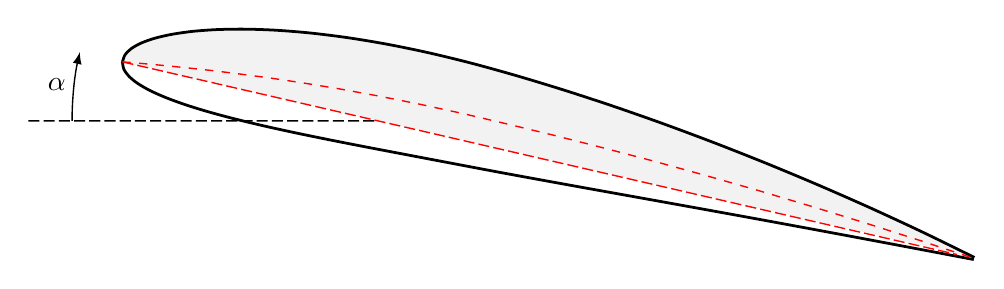
\begin{tikzpicture}[>=latex,scale=1.11]
\tikzstyle{spring}=[snake=zigzag,thick,line before snake=0.3cm,line after  snake=0.3cm,segment length=6,segment amplitude=5,join=round]%
\begin{scope}[rotate around={-13:(10,0)}]
% bottom_second
\draw[smooth,line width=1pt] plot coordinates {(0,0)(0.0334,-0.0767)(0.1087,-0.1437)(0.2253,-0.2011)(0.3824,-0.2489)(0.5790,-0.2870)(0.8139,-0.3158)(1.0860,-0.3355)(1.3940,-0.3466)(1.7365,-0.3497)(2.1123,-0.3457)(2.5199,-0.3356) (2.9580,-0.3209)(3.4252,-0.3029)(3.9198,-0.2835)(4.4427,-0.2625)(4.9936,-0.2377)(5.5666,-0.2102)(6.1594,-0.1810)(6.7696,-0.1513)(7.3950,-0.1217)(8.0332,-0.0930)(8.6815,-0.0653)(9.3376,-0.0386)(9.9988,-0.0125)};
% top_first
\draw[smooth,line width=1pt,fill=black!5] plot coordinates {(0,0)(0.0095,0.0831)(0.0624,0.1691)(0.1590,0.2574)(0.2990,0.3467)(0.4824,0.4357)(0.7085,0.5225)(0.9765,0.6050)(1.2855,0.6812)(1.6341,0.7488)(2.0206,0.8055)(2.4433,0.8492)(2.8998,0.8778)(3.3879,0.8897)(3.9049,0.8833)(4.4459,0.8592)(5.0064,0.8210)(5.5876,0.7687)(6.1870,0.7023)(6.8016,0.6219)(7.4286,0.5277)(8.0650,0.4197)(8.7080,0.2980)(9.3544,0.1623)(10.0012,0.0125)};
% sekelett
\draw[dashed, color=red, line width=0.5pt] plot coordinates { (0.0, 0.0)(0.021, 0.003)(0.086, 0.013)(0.192, 0.028)(0.341, 0.049)(0.531, 0.074)(0.761, 0.103)(1.031, 0.135)(1.34, 0.167)(1.685, 0.2)(2.066, 0.23)(2.482, 0.257)(2.929, 0.278)(3.407, 0.293)(3.912, 0.3)(4.444, 0.298)(5.0, 0.292)(5.577, 0.279)(6.173, 0.261)(6.786, 0.235)(7.412, 0.203)(8.049, 0.163)(8.695, 0.116)(9.346, 0.062)(10.0, 0.0) };
\draw[line width=0.5pt,dashed,dash pattern=on 4pt off 1.5pt,rotate around={13:(3,0)}](-1,0)--(3,0);
% arrows
\draw[line width=0.5pt,<-](3,0) +(180:3.5cm) arc (180:193:3.5cm);
\draw(3,0) +(186.5:3.7cm) node{$\alpha$};
% sehne
\draw[line width=0.5pt,color=red, dashed,dash pattern=on 4pt off 1.5pt](0,0)--(9.8,0);
\end{scope}%
\end{tikzpicture}
\endpgfgraphicnamed%



\begin{tikzpicture}
% profile with data file
%\newcounter{y}
\setcounter{y}{0}
\foreach \x in {1.00}
    \draw (11 cm,1pt) -- (11 cm,-1pt) node[anchor=north] {$\x$};
    \draw (1pt,0 cm) -- (-1pt,0 cm) node[anchor=east] {$0$};
	\draw (1pt,1.25 cm) -- (-1pt,1.25 cm) node[anchor=east] {$0.10$};
	\draw (1pt,-1.25 cm) -- (-1pt,-1.25 cm) node[anchor=east] {$-0.10$};
    \foreach \lbl / \fn in {naca4815.dat}{
        % Some profiles look better when using plot[smooth]
        \draw[yshift=-\arabic{y}cm,scale=11, fill=black!5]% node[left=0.5cm] {\lbl}
            plot file{tikz/data/\fn} -- cycle;
        \stepcounter{y}
    }
% axis
\draw[thick,-] (0,0)  -- (12,0) node[anchor=west] {x};
\draw[thick,-] (0,-2) -- (0,2) node[anchor=south] {y};    
% camber line    
\draw[smooth, dashed, scale=11] plot coordinates {(1.0,0.0)(0.998459,0.000614)(0.993844,0.0024245)(0.986185,0.0053355)(0.975528,0.00919)(0.96194,0.0137755)(0.945503,0.018829)(0.92632,0.0240435)(0.904508,0.029078)(0.880203,0.0335675)(0.853553,0.037132)(0.824724,0.039389)(0.793893,0.0399975)(0.761249,0.0399065)(0.726995,0.039667)(0.691342,0.039262)(0.654508,0.038677)(0.616723,0.037901)(0.578217,0.036926)(0.53923,0.03575)(0.5,0.034375)(0.46077,0.0328075)(0.421783,0.0310595)(0.383277,0.0291465)(0.345492,0.0270885)(0.308658,0.0249115)(0.273005,0.022642)(0.238751,0.0203125)(0.206107,0.0179555)(0.175276,0.0156075)(0.146447,0.013304)(0.119797,0.0110825)(0.095492,0.008979)(0.07368,0.0070285)(0.054497,0.005264)(0.03806,0.0037155)(0.024472,0.0024095)(0.013815,0.0013695)(0.006156,0.000613)(0.001541,0.000154)(0.0,0.0)};    	
\end{tikzpicture}    


\begin{tikzpicture}
% axis
\draw[thick,-] (11,0)  -- (12,0) node[anchor=west] {x};
\draw[thick,-] (0,-2) -- (0,2) node[anchor=south] {y};
% profile with data file
%\newcounter{y}
\setcounter{y}{0}
\foreach \x in {1.00}
    \draw (11 cm,1pt) -- (11 cm,-1pt) node[anchor=north] {$\x$};
    \draw (1pt,0 cm) -- (-1pt,0 cm) node[anchor=east] {$0$};
	\draw (1pt,1.25 cm) -- (-1pt,1.25 cm) node[anchor=east] {$0.10$};
	\draw (1pt,-1.25 cm) -- (-1pt,-1.25 cm) node[anchor=east] {$-0.10$};
    \foreach \lbl / \fn in {naca4815.dat}{
        % Some profiles look better when using plot[smooth]
        \draw[yshift=-\arabic{y}cm,scale=11]% node[left=0.5cm] {\lbl}
            plot file{tikz/data/\fn} -- cycle;
        \stepcounter{y}
    }
% camber line    
\draw[smooth, dashed, color=red, scale=11] plot coordinates {(1.0,0.0)(0.998459,0.000614)(0.993844,0.0024245)(0.986185,0.0053355)(0.975528,0.00919)(0.96194,0.0137755)(0.945503,0.018829)(0.92632,0.0240435)(0.904508,0.029078)(0.880203,0.0335675)(0.853553,0.037132)(0.824724,0.039389)(0.793893,0.0399975)(0.761249,0.0399065)(0.726995,0.039667)(0.691342,0.039262)(0.654508,0.038677)(0.616723,0.037901)(0.578217,0.036926)(0.53923,0.03575)(0.5,0.034375)(0.46077,0.0328075)(0.421783,0.0310595)(0.383277,0.0291465)(0.345492,0.0270885)(0.308658,0.0249115)(0.273005,0.022642)(0.238751,0.0203125)(0.206107,0.0179555)(0.175276,0.0156075)(0.146447,0.013304)(0.119797,0.0110825)(0.095492,0.008979)(0.07368,0.0070285)(0.054497,0.005264)(0.03806,0.0037155)(0.024472,0.0024095)(0.013815,0.0013695)(0.006156,0.000613)(0.001541,0.000154)(0.0,0.0)};  
% sehne
\draw[line width=0.5pt,color=red](0,0)--(11,0);    	
\end{tikzpicture} 
	\caption{Eine Vektorgrafik}
	\label{fig:vectorExample}
\end{figure}










\subsection{Rumpfprofile}
\blindtext






%\newpage
%\newpage\thispagestyle{empty}\hspace{1em}\newpage
\chapter{Eigenes Verfahren}
In diesem Kapitel soll das eigene Verfahren beschrieben werden. Es geht dabei nicht nur darum zu beschreiben was gemacht wurde, sondern ebenfalls darum zu begr�nden, weshalb bestimmte Design-Entscheidungen getroffen wurden.


\section{LaTex-Editoren}

Ein guter Cross-Plattform (Windows/Linux/Mac) Latex-Editor mit englischer und deutscher Rechtschreibkorrektur ist z.B. TexStudio
(\url{http://texstudio.sourceforge.net/}). Unter Windows verwende ich diesen Editor gerne zusammen mit dem Sumatra PDF Viewer (\url{http://blog.kowalczyk.info/software/sumatrapdf/free-pdf-reader.html}), da dieser ein automatisches Neuladen unterst�tzt.

%%%%%%%%%%%%%%%%%%%%%%%%%%%%%%%%%%%%%%%%%%%%%%%%%%%%%%%%%%%%%%%%%%%%%%%%%%%%%%%%%%%%%%%%%%%%%%%%%%%%%%%%%%%%%%%%%%%%%%%%%
\section{Beispiel f�r eine Tabelle}
In Tabelle \ref{tab:bibliotheken} sind die verwendeten Bibliotheken ausgelistet.
\begin{table}[htbp]
\centering 
\begin{tabular}{ll}
\toprule \textbf{Bibliothek} & \textbf{Version} \\
\bottomrule
CUDA SDK & 2.3 \\
CUDA Toolkit & 2.3 \\
 OpenGL & 3.2 \\
 GLUT & 3.7 \\
GLEW & 1.5.1 \\
CUDPP & 1.1 \\
\bottomrule
\end{tabular}
\caption{Die verwendeten Bibliotheken.}
\label{tab:bibliotheken}
\end{table}

\section{Formel in Latex und Konventionen zur Verwendung mathematischer Symbole}
Mathematische Symbole k�nnen in Latex sehr leicht erzeugt werden. Beispiel f�r Symbole im Text: Gegeben sei ein Skalar $a \in \mathbb{R}$. Tabelle~\ref{tab:mathematischeSymbole} liste einige Konventionen zur Verwendung mathematischer Symbole. Abgesetzte Formel lassen sich ebenfalls leicht erzeugen:
\begin{equation}
\label{eqn:beispiel}
f(x) = x^2 + 3
\end{equation}
Au�erdem kann leicht auf abgesetzte Formel verwiesen werden (siehe Gleichung~\ref{eqn:beispiel}). F�r mehrere ausgerichtete Formeln bietet sich die Umgebung \texttt{eqnarray} an:
\begin{eqnarray}
\label{eqn:beispiel2}
f(x) &=& x^2 + 3 \\
g(\theta) &=& \cos (2\theta) = \cos^2 \theta - \sin^2 \theta\\
h(x) &=& \int_0^\infty \mathrm{e}^{-x}\,\mathrm{d}x
\end{eqnarray}


\begin{table}[htbp]
\centering
\begin{tabular}{lll}
\toprule \textbf{Typ} & \textbf{Schriftart} & \textbf{Beispiele} \\
\bottomrule
Variablen (Skalare) & kursiv & $a, b, x, y$ \\
Funktionen & aufrecht& $\mathrm{f}, \mathrm{g}(x), \mathrm{max}(x)$\\
Vektoren & fett, Elemente zeilenweise & $\mathbf{a}, \mathbf{b}= \begin{pmatrix}x\\y\end{pmatrix} = (x, y)^\top$\\
Matrizen & Schreibmaschine& $\mathtt{A}, \mathtt{B}= \begin{bmatrix}a & b\\c & d\end{bmatrix}$\\
Mengen & kalligrafisch& $\mathcal{A}, \{a, b\} \in \mathcal{B}$ \\
Zahlenbereiche & doppelt gestrichen& $\mathbb{N}, \mathbb{Z}, \mathbb{R}^2, \mathbb{R}^3$ \\
\bottomrule
\end{tabular}
\caption{Konventionen zur Verwendung mathematischer Symbole}
\label{tab:mathematischeSymbole}
\end{table}






\section{Beispiel f�r eine Vektorgrafik}

Wenn m�glich sollten immer Vektorgrafiken verwendet werden. Rastergrafiken sollten nur dann eingesetzt werden, wenn die Original-Quelle ebenfalls eine Rastergrafik ist. Ein 
Cross-Plattform Editor zur Erstellung von Vektorgrafiken ist z.B. Inkscape:
\url{http://inkscape.org/download/}. Nach der Erstellung in Inkscape sollte die Grafik zum einen zur sp�teren Weiterverarbeitung als SVG gespeichert werden. Zum anderen zwecks Import in Latex als PDF. Abbildung~\ref{fig:vectorExample} zeigt ein Beispiel.


\begin{figure}[htpb]
	\centering
		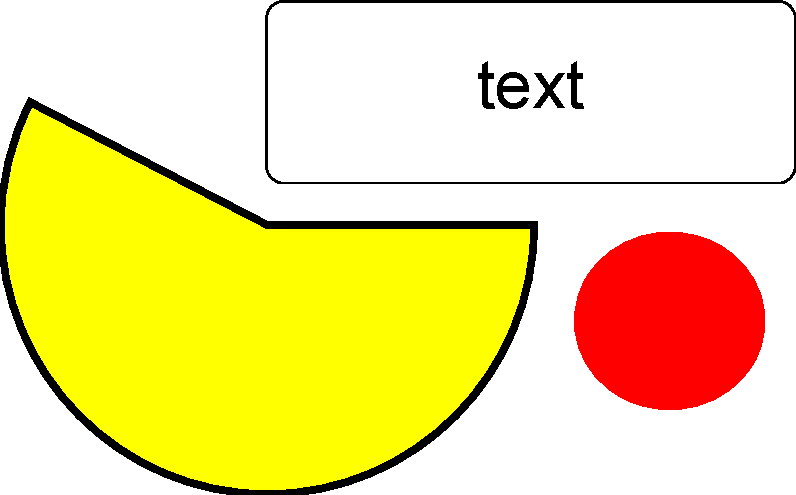
\includegraphics[width=0.30\textwidth]{fig/vectordrawing.pdf}
	\caption{Eine Vektorgrafik}
	\label{fig:vectorExample}
\end{figure}


\section{Beispiel f�r eine Vektorgrafik mit mathematischen Symbolen}

Um beliebigen Latex-Code in eine Vektorgrafik einzuf�gen (z.B. um mathematische Symbole zu setzen) kann in Inkscape beim Speichern der Datei als PDF die Option \glqq Pdf+Latex: Text in PDF weglassen und Latex Datei erstellen\grqq  ~angew�hlt werden (siehe Abb.~\ref{fig:vectorExampleSymbol})

\begin{figure}[htpb]
    \centering
    \def\svgwidth{0.30\textwidth}
  	\import{./fig/}{vectordrawingSymbol.pdf_tex}
	\caption{Eine Vektorgrafik mit mathematischen Symbolen}
	\label{fig:vectorExampleSymbol}
\end{figure}

\section{Beispiel f�r eine Rastergrafik}

Abbildung~\ref{fig:exampleFigure} zeigt, wie eine Rastergrafik eingebunden werden kann. \\

\begin{figure}[htpb]
    \centering
  	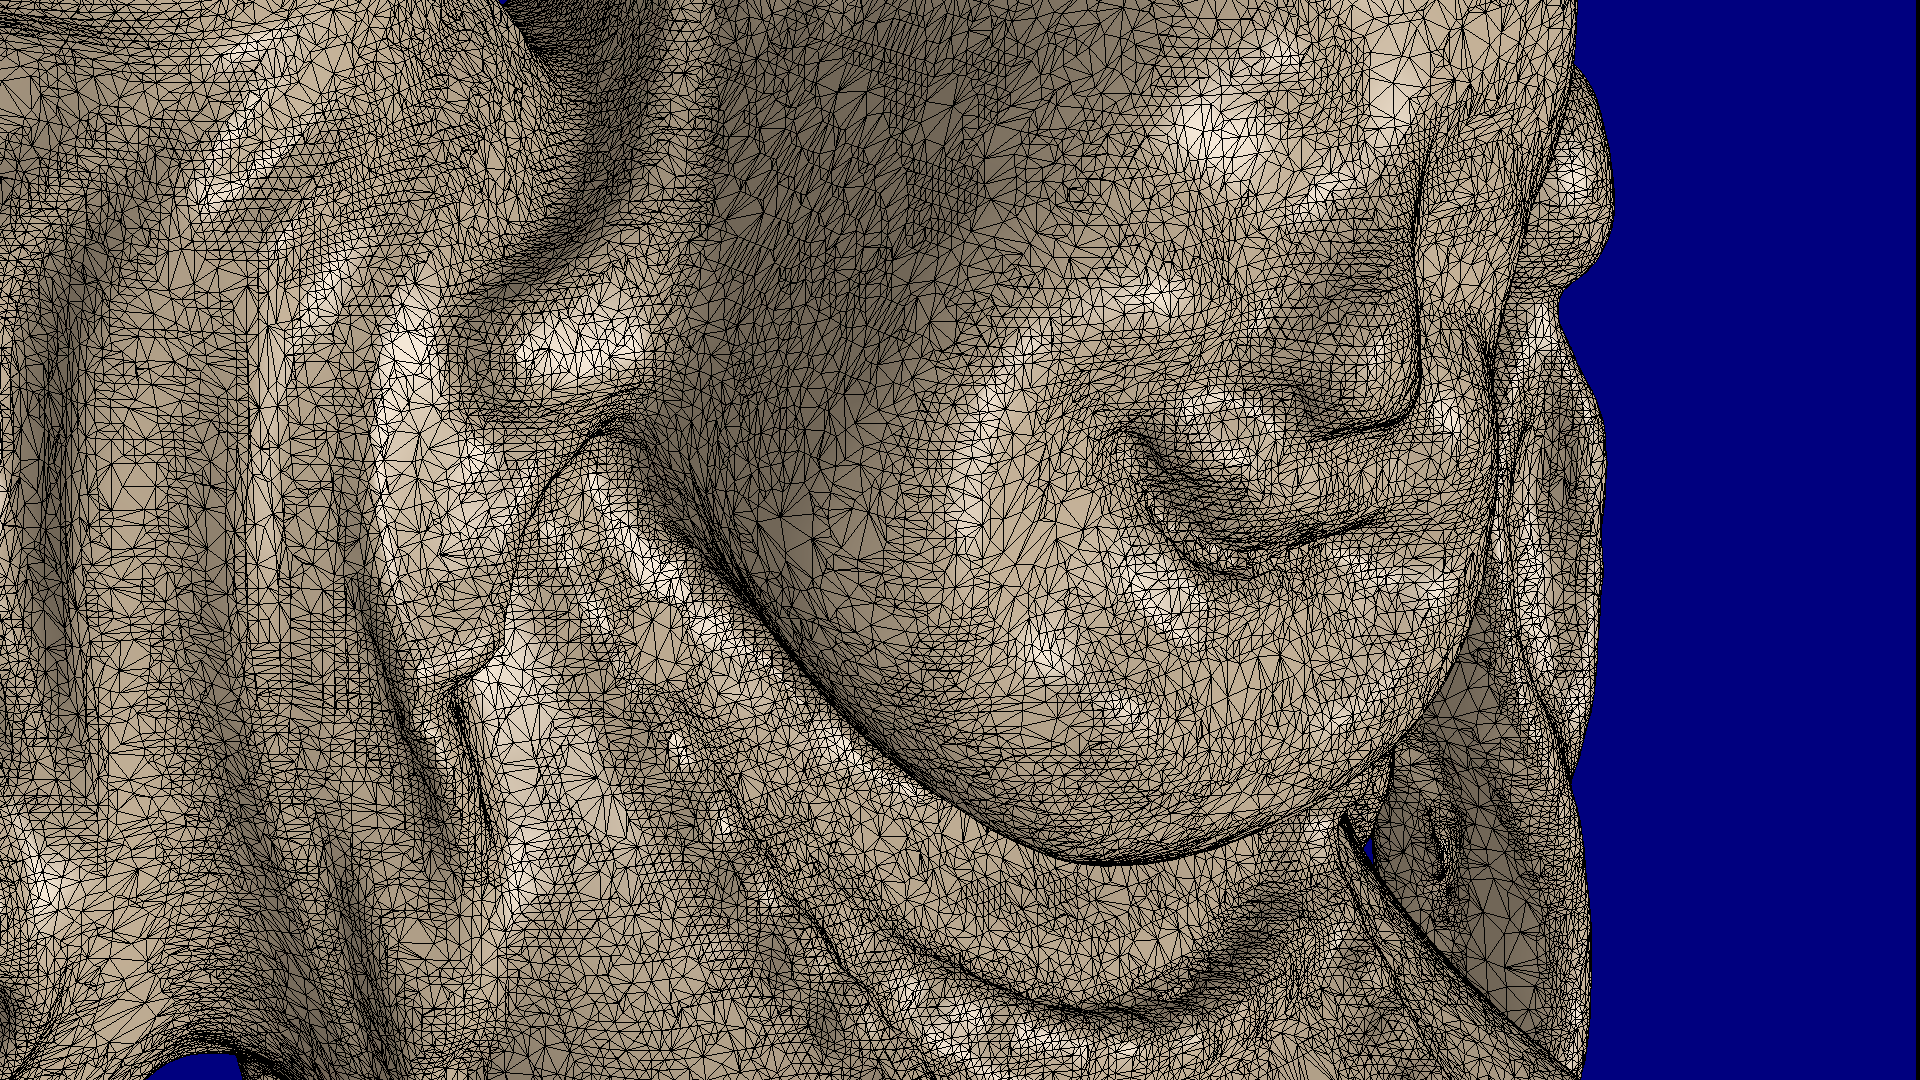
\includegraphics[width=0.80\textwidth]{fig/Buddha2.png}
	\caption{Eine Rastergrafik}
	\label{fig:exampleFigure}
\end{figure}


Bild- bzw. Tabellen-Beschriftungen sollten m�glichst informativ sein. Aus der Beschreibung sollte die Bedeutung der Abbildung vollst�ndig hervorgehen, so dass der Haupttext zum Verst�ndnis nicht notwendigerweise gelesen werden muss. 

\newpage
\section{Beispiel f�r die Darstellung von Algorithmen}

Algorithmus \ref{algo:algorithmSCAN} zeigt ...

\begin{algorithm}[htpb]
	\textit{Phase 1: Reduktion}\\
	\texttt{for} $d := 0$ \texttt{to} $log_2 n - 1$ ~\texttt{in parallel do}\\
	\hspace{5mm}\texttt{for} $k := 0$ \texttt{to} $n - 1$ \texttt{by} $2^{d+1}$ ~\texttt{in parallel do}\\
	\hspace{10mm}$x[k + 2^{d + 1} - 1] := x[k + 2^d - 1] + x [k + 2^{d + 1} - 1]$\\
	\textit{Phase 2: Propagation}\\
	\texttt{for} $d := log_2 n$ \texttt{to} $0$ ~\texttt{in parallel do}\\
	\hspace{5mm}\texttt{for} $k := 0$ \texttt{to} $n - 1$ \texttt{by} $2^{d+1}$ ~\texttt{in parallel do}\\
	\hspace{10mm}$t := x[k + 2^d - 1]$\\
	\hspace{10mm}$x[k + 2^d - 1] := x [k + 2^{d + 1} - 1]$\\
	\hspace{10mm}$x[k + 2^{d + 1} - 1] := t + x [k + 2^{d + 1} - 1]$\\
	\caption{Pseudocode der zwei Phasen vom SCAN-Algorithmus \cite{bib:SCAN}.}
	\label{algo:algorithmSCAN}
\end{algorithm}

\section{Beispiel f�r die Darstellung von Quellcode-Ausz�gen}

dies ist \verb+'+ \LaTeX

Listing \ref{lst:VBOkontrolle} zeigt ...
\lstinputlisting[language=Python, float=htpb, caption={Pseudocode f�r die Kontrolle der VBOs}, label=lst:VBOkontrolle, captionpos=b, keywordstyle=\bfseries\color{black}]{code/test.py}


Listing \ref{lst:VBOkontrolle} zeigt ...
\lstinputlisting[language=Python, style=customc, float=htpb, caption={Pseudocode f�r die Kontrolle der VBOs}, label=lst:VBOkontrolle, captionpos=b, keywordstyle=\bfseries\color{black}]{code/test.py}


Listing \ref{lst:VBOkontrolle} zeigt ...
\lstinputlisting[language=Python, style=customc, float=htpb, caption={Pseudocode f�r die Kontrolle der VBOs}, label=lst:VBOkontrolle, captionpos=b, keywordstyle=\bfseries\color{black}]{code/test2.py}


\section{Hier ein uml diagramm}
\begin{tikzpicture}
\umlemptyclass[width=15ex]{class20}
\umlemptyclass[y=2, width=30ex]{class40}
\end{tikzpicture}


\section{hier kommt pstricks}

\begin{figure}[h]
\centering
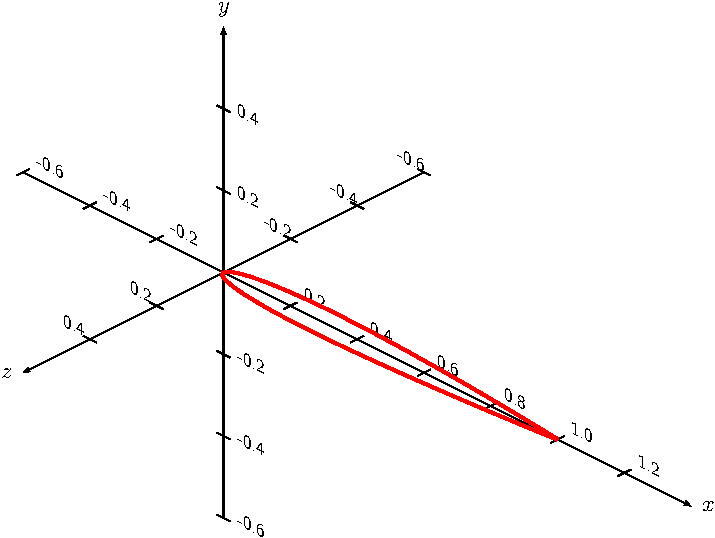
\includegraphics[width=0.7\linewidth]{tikz/Airfoil-crop}
\caption{Mein erster Funktionsplot PSTricks}
\end{figure} %% --> Leerzeile danach wichtig

\begin{figure}[h]
\centering
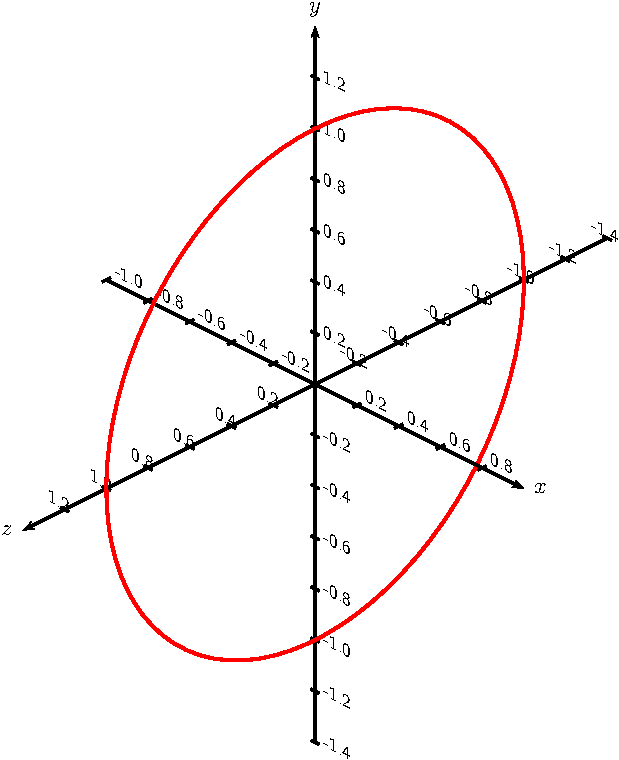
\includegraphics[width=0.7\linewidth]{tikz/Fuselage-crop}
\caption{Mein erster Funktionsplot PSTricks}
\end{figure} %% --> Leerzeile danach wichtig

%\newpage
%\newpage\thispagestyle{empty}\hspace{1em}\newpage
%\chapter{Ergebnisse und Evaluation}
In diesem Kapitel sollen die Ergebnisse dieser Diplomarbeit diskutiert werden. 




%\newpage
%\newpage\thispagestyle{empty}\hspace{1em}\newpage
\chapter{Zusammenfassung und Ausblick}
In diesem Kapitel sollen zun�chst die erreichten Ziele diskutiert und abschlie�end ein Ausblick auf m�gliche, weiterf�hrende Arbeiten gegeben werden.

\newpage
\pagenumbering{Roman}
\setcounter{page}{1}

\nocite{*}%Auch nicht-zitierte BibTeX-Eintr�ge werden angezeigt.
\bibliography{chapters/Literaturverzeichnis}
\bibliographystyle{eg-alpha}
\newpage
\newpage\thispagestyle{empty}\hspace{1em}\newpage
\chapter*{Abk�rzungsverzeichnis}
\begin{acronym}[PM]
 %Sorgt daf�r, dass zwischen den Eintr�gen kein Abstand ist und das Verzeichnis kompakt dargestellt wird.
 \setlength{\itemsep}{-\parsep}
 \acro{ALU}{Arithmetic Logic Unit}
 \acro{BTF}{Bidirektionalen Textur Funktion}
 \acro{CPU}{Central Processing Unit}
 \acro{CU}{Control Unit}
 \acro{CUDA}{Compute Unified Device Architecture}
 \acro{FLOPs}{Floating Point Operations Per Second}
 \acro{FPU}{Floating Point Unit}
 \acro{GPGPU}{General Purpose Compution on Graphics Processing Unit}
 \acro{GPU}{Graphics Processing Unit}
 \acro{HLOD}{Hierarchische Level of Detail}
 \acro{IFS}{Indexed-Face-Set}
 \acro{LOD}{Level of Detail}
 \acro{MIMD}{Multiple Instruction Multiple Data}
 \acro{OpenCL}{Open Computing Language}
 \acro{OpenGL}{Open Graphics Library}
 \acro{PCAM}{Partitionierung Kommunikation Agglomeration Mapping}
 \acro{PM}{Progressive Meshes}
 \acro{SFU}{Spezial Funktion Units}
 \acro{SIMD}{Single Instruction Multiple Data}
 \acro{SIMT}{Single Instruction Multiple Threads}
 \acro{SLI}{Scalable Link Interface}
 \acro{SP}{Streaming-Prozessoren}
 \acro{SM}{Streaming-Multiprozessoren}
 \acro{TPC}{Textur Prozessor Clustern}
 \acro{VBO}{Vertex Buffer Object}

 
\end{acronym}

%Abk�rzungsverzeichnis im Inhaltsverzeichnis anzeigen
\addcontentsline{toc}{chapter}{Abk�rzungsverzeichnis} 
%Abbildungsverzeichnis
\newpage\thispagestyle{empty}\hspace{1em}\newpage
\listoffigures
%Tabellenverzeichnis
\listoftables
%Liste von Algorithmen
\newpage\thispagestyle{empty}\hspace{1em}\newpage
\markboth{Liste der Algorithmen}{Liste der Algorithmen}
\phantomsection
\addcontentsline{toc}{chapter}{Liste der Algorithmen}
\listofalgorithms
%Liste von Code
\newpage\thispagestyle{empty}\hspace{1em}\newpage
\markboth{Listings}{Listings}
\phantomsection
\addcontentsline{toc}{chapter}{Listings}
\lstlistoflistings
%Anhang
\newpage
\newpage\thispagestyle{empty}\hspace{1em}\newpage
\appendix
\chapter{Anhang}\label{chp:AnhangA}
\section*{Thema 1}\label{sec:AnhangA1}

Beispiel f�r einen Anhang

\section*{Thema 2}\label{sec:AnhangA2}

%Danksagung
\chapter*{Danksagung}
Hiermit m�chte ich mich besonders bei Prof. Dr. XXXX, Prof. Dr. xxxx, Dipl. Inf. xxxx und Dipl. Inf. xxx f�r die Betreuung meiner Arbeit, hilfreiche Diskussionen und viel Geduld bei zahlreichen Fragen bedanken.
\end{document} | returns and the picture is ready. From this point on, the external graphics will be used.

There is another possibility to communicate \meta{main document} to the subprocess performing the externalization: namely to write `|\tikzexternalize{main}|' into the document. In this case, the conversion system call will be
\begin{codeexample}[code only, tikz syntax=false]
pdflatex -jobname "main-figure0" "main"
\end{codeexample}
\noindent and the contents of |\tikzexternalrealjob| is set automatically. This case is detected by |\tikzexternalize|, and the |system call| is updated automatically (by patching its |\texsource| template argument). It is not necessary to change the |system call| manually.


The sequence in which system calls are performed and the decision whether they are issued automatically is governed by the |mode| key, consult its documentation for details.


\subsection{Using External Graphics Without \textmd{\pgfname}\ Installed}
\label{section-libs-external-nopgf}
Given that every picture has been exported correctly, one may want to compile a file without \pgfname\ and \tikzname\ installed. \tikzname\ comes with a minimal package which contains just enough commands to replace every |tikzpicture| environment and the |\tikz| short command with the appropriate external graphics. It can be found at
\begin{codeexample}[code only, tikz syntax=false]
latex/pgf/utilities/tikzexternal.sty
\end{codeexample}
\noindent and needs to be used instead of |\usepackage{tikz}|. So, we uncomment |\usepackage{tikz}| and our example from the beginning becomes
\begin{codeexample}[code only]
\documentclass{article}
% main document, called main.tex
%\usepackage{tikz}

\usepackage{graphicx}
\usepackage{tikzexternal}

%\usetikzlibrary{external}
\tikzexternalize

\begin{document}
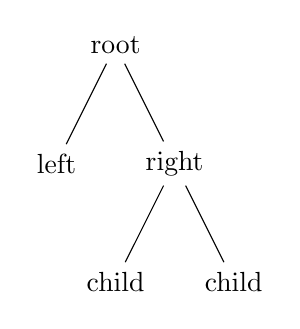
\begin{tikzpicture}
  \node {root}
    child {node {left}}
    child {node {right}
      child {node {child}}
      child {node {child}}
    };
\end{tikzpicture}

A simple image is \tikz \fill (0,0) circle(5pt);.

Furthermore, we might want to draw \tikz[baseline]\draw (0,-1) rectangle (1,1);
\end{document}
\end{codeexample}
\noindent where the following files are necessary to compile the document:
\begin{codeexample}[code only, tikz syntax=false]
tikzexternal.sty
main.tex
main-figure0.pdf
main-figure1.pdf
main-figure2.pdf
\end{codeexample}
\noindent If there are any `|.dpth|' files, for example |main-figure2.dpth|, these files are also required. They contain information for the \tikzname\ |baseline| option (or |\label|s inside external graphics).

Just copy the |.sty| file into the directory of your |main.tex| file and use it as part of your document.

Please keep in mind, that only |tikzpicture| environments and |\tikz| short images are available within the externalization framework. Additionally, calls to |\tikzset| and |\pgfkeys| won't lead to compilation errors because they are simply ignored. But since |pgfkeys| is not available, any option supplied to |\tikzexternalize| is \emph{ignored}.

\paragraph{Attention:} Since the simple replacement |\usepackage{tikzexternal}| doesn't support the key--value interface, you \emph{need} to use |\tikzsetexternalprefix| instead of the |prefix| option and |\tikzsetfigurename| instead of the |figure name| option since |\tikzset| is not available in such a context.

\paragraph{Remark:} Some of the features of this library are mainly useful to improve the speed of successive document compilations. In other words: you can't use all features in this context, keep it simple.

\subsection{\eps\ Graphics Export}
It is also possible to use \eps\ graphics instead of \pdf\ files. There are different ways to produce them, for example to use |pdflatex| and call |pdftops -eps |\marg{pdf file} \marg{eps file} afterwards. You could add this command to the |system call| option.

Alternatively, you can use |latex| and |dvips| for image conversion as is explained for the |system call| option, see page~\pageref{extlib:systemcall:option}. See the documentation for the basic level externalization in section~\ref{section-external} for restrictions of other drivers.

\subsection{Bitmap Graphics Export}
Occasionally, you may have an extremely large graphics which takes long times to render. It might be interesting to generate a bitmap (raster) image, which displays much faster (for example in a presentation). I have used this feature to speed-up the display of large shadings.

The |external| library can be customized to export bitmap images -- with the help of external programs. Due to the dependence of external programs, you may need to adjust these commands manually. For example, on my computer, the ImageMagick Suite is installed which comes with the |convert| tool. Together with |pdflatex|, I can define the following style:
\begin{codeexample}[code only]
\tikzset{
    % Defines a custom style which generates BOTH, .pdf and .png export
    % but prefers the .png on inclusion.
    %
    % This style is not pre-defined, you may need to copy-paste and
    % adjust it.
    png export/.style={
        external/system call/.add=
            {}
            {; convert -density 300 -transparent white "\image.pdf" "\image.png"},
        %
        /pgf/images/external info,
        /pgf/images/include external/.code={%
            \includegraphics
                [width=\pgfexternalwidth,height=\pgfexternalheight]
                {##1.png}%
        },
    }
}
\end{codeexample}
\noindent The example above defines a new style called `|png export|' which, when it is set with |\tikzset{png export}| somewhere in the document, modifies the configuration for both file generation and file input. The file generation is modified by appending the ImageMagick command to |system call| (separated by `|;|' as usual on Linux). This is, in principle, enough to generate a |.png| file. The |include external| command is overwritten such that it uses the |.png| file instead of the |.pdf| file (which exists as well in the configuration above). But since a |.png| file can have a much higher resolution than the desired image dimensions, we have to add |width| and |height| explicitly. Usually, the |external| library does not provide size information (it is unnecessary for |.pdf| or |.eps| since these formats have their bounding box information). To enable size information, the style uses the |external info| key, which, in turn, provides the |\pgfexternalwidth| and |\pgfexternalheight| commands.

Now we can use |\tikzset{png export}| either document-wide or just for one particular image. The configuration remains in effect until the end of the current environment (or until the next closing curly brace `|}|').

\begin{key}{/pgf/images/external info=\marg{boolean} (initially false)}
	If this key is activated, the size for any externalized image will be stored explicitly into the associated |.dpth| file.

	When the file is included by |\pgfincludeexternalgraphics| (or automatically by the |external| library), the width is available as \declareandlabel{\pgfexternalwidth} and the height as \declareandlabel{\pgfexternalheight}.
\end{key}

\subsection{Compatibility Issues}
\subsubsection{References In External Pictures}
It is allowed if a picture contains references, for example |\tikz \node {Reference to \ref{a:label}};|.

There is just one issue: if the main job is currently compiling, its |.aux| file is not in its final state (even worse: it may not be readable at all). The picture externalization, however, needs the main |.aux| file to query any references.

Thus, you \emph{will} need to invoke |pdflatex -jobname |\meta{image}| |\meta{mainfile} \emph{manually} for any image which contains references.

This problem arises only for |mode=convert with system call|. In this case,  the |external| library creates a special |\jobname.auxlock| file to check whether the main |.aux| file is currently usable.

\subsubsection{Compatibility With Other Libraries or Packages}
The |external| library has the following compatibility issues:
\begin{enumerate}
	\item The |external| library comes with special support for |\usetikzlibrary{fadings}|: the |fadings| library may define local pictures which would be externalized (although they shouldn't). There is special handling to suppress this bug if |\tikzexternalize| is called \emph{after} |\usetikzlibrary{fadings}| or if all fadings are defined \emph{before} |\tikzexternalize|.

	\item Problems have been reported when using |\tikzexternalize| (or the basic layer externalization) together with |\usepackage{glossary}|. This problem disappears if |\tikzexternalize| is called \emph{before} |\usepackage{glossary}|.

	\item Problems with |\usepackage{pdfpages}| and |\usepackage{vmargin}|: The |external| library replaces the current shipout routine of \TeX\ during its externalization. This might raise problems with other packages which also manipulate the shipout routine (like the mentioned ones).

	To fix those problems, use
\begin{codeexample}[code only]

\usetikzlibrary{external}

\tikzifexternalizing{%
	% don't include package XYZ here
}{%
	\usepackage{pdfpages}
	\usepackage{vmargin}
	...
}%
\end{codeexample}
	This uses the requested packages for the main document, but not for the single, exported graphics.
\end{enumerate}

In general, the |\tikzifexternalizing| feature might be used to solve package conflicts and the |\tikzexternaldisable| and |\tikzexternalenable| features can be used to solve problems with single pictures.

\subsubsection{Compatibility With Bounding Box Restrictions}
Bounding box restrictions provide no problem when used with \eps\ graphics. However, they pose problems for |pdflatex|, so you may need to use the |latex| / |dvips| combination if you use bounding box restrictions and externalization. Currently, the only possibility for bounding box restrictions and |pdflatex| is to use a combination of |trim left| / |trim right| / |baseline|: these keys do not \emph{really} truncate the bounding box, they only store horizontal and vertical shifts (also see the |trim lowlevel| key in this context).

\subsubsection{Interoperability With The Basic Layer Externalization}
This library is fully compatible with |\beginpgfgraphicnamed|$\dotsc$|\endpgfgraphicnamed| environments. However, you will need to use the |export next=false| key to avoid conflicts:
\begin{codeexample}[code only]
\beginpgfgraphicnamed{picture4}
\tikzset{external/export next=false}
\begin{tikzpicture}
   \draw (0,0) -- (4,4);
\end{tikzpicture}
\endpgfgraphicnamed
\end{codeexample}
Please keep in mind that file prefixes do not apply to the basic layer.
}
\endinput
